\documentclass[12pt]{report}

%\usepackage[UTF8]{ctex}
%\usepackage{CJKutf8}
%\usepackage[noconfigs,english]{babel}

\usepackage{xeCJK}
%\setCJKmainfont{SimHei}
\setCJKmainfont{SimSun}

\usepackage{graphicx}
\graphicspath{{figures/}}
\usepackage{latexsym}
\usepackage{amsmath}
\usepackage{amssymb}
\usepackage{hyperref}
\hypersetup{
     breaklinks,
     colorlinks   = true,
     citecolor    = blue,
     linkcolor    = red
}

%\usepackage[]{natbib}
\usepackage{lscape}
\usepackage{bm}
\usepackage{mathrsfs}
\usepackage{booktabs}
\usepackage[capitalise]{cleveref}
\crefname{figure}{Fig.}{Figs.}
\Crefname{figure}{Fig.}{Figs.}

\ExecuteOptions{dvips} \marginparwidth 0pt \oddsidemargin 0.5 truecm
\evensidemargin 1.5 truecm \marginparsep 0pt \topmargin 0pt
\textheight 22.0 truecm \textwidth 14.5 truecm
\renewcommand{\baselinestretch}{1.5}

\newcommand{\chapterend}{
	\vfill
	\noindent\rule{\textwidth}{0.5mm} \\
	\noindent{\large\bf $\Box$ End of chapter.}
}

\newcommand*{\mkred}[1]{{\color{red}{#1}}}
\def\question{{\color{red}{(?)}}}
\usepackage{array}


%===============

\usepackage{fancyhdr}  
\usepackage{lastpage}                                           
\usepackage{layout}   
%=======================================================

\def\d{\textrm{d}}
\def\be{\begin{equation}}
\def\ee{\end{equation}}
\def\({\left(}
\def\){\right)}
\def\[{\left[}
\def\]{\right]}
\def\<{\left<}
\def\>{\right>}
\def\nn{\nonumber}

\newcommand{\IMRP}{\texttt{IMRPhenomPv2}}
\newcommand{\IMRB}{\texttt{IMRPhenomB}}
\newcommand{\IMRA}{\texttt{IMRPhenomA}}
\newcommand{\IMRD}{\texttt{IMRPhenomD}}
\newcommand{\IMRN}{\texttt{IMRPhenomD-NRTidal}}
\newcommand{\LAL}{\texttt{LALSuite}}
\newcommand{\linf}{\textsc{LALInference}}
\newcommand{\BW}{\textsc{BayesWave}}
\newcommand{\BL}{\textsc{BayesLine}}
\newcommand{\PYCBC}{\textsc{PyCBC}}

\usepackage{acro}
\DeclareAcronym{EMRI}{
	short = EMRI,
	long  = extreme mass ratio inspiral
}
\DeclareAcronym{PTA}{
	short = PTA,
	long  = pulsar timing array
}

\DeclareAcronym{LISA}{
	short = LISA,
	long  = Laser Interferometer Space Antenna
}

\DeclareAcronym{GR}{
	short = GR,
	long  = general relativity
	}
	
\DeclareAcronym{BH}{
	short = BH ,
	long  = black hole
}
\DeclareAcronym{PBH}{
	short = PBH ,
	long  = primordial black hole
}
\DeclareAcronym{SGWB}{
	short = SGWB ,
	long  = stochastic gravitational-wave background
}
\DeclareAcronym{BBH}{
	short = BBH ,
	long  = binary black hole
}
\DeclareAcronym{BNS}{
	short = BNS ,
	long  = binary neutron star
}
\DeclareAcronym{NSBH}{
	short = NSBH ,
	long  = neutron star black hole
}

\DeclareAcronym{GW}{
	short = GW ,
	long  = gravitational wave
}
\DeclareAcronym{CMB}{
	short = CMB ,
	long  = cosmic microwave background
} 
\DeclareAcronym{SFR}{
	short = SFR ,
	long  = star formation rate
}

\DeclareAcronym{CBC}{
	short = CBC,
	long  = compact binary coalescence
}
\DeclareAcronym{SNR}{
	short = SNR,
	long  = signal noise ratio
}
\DeclareAcronym{IMR}{
	short = IMR,
	long  = inspiral-merger-ringdown
}

\DeclareAcronym{KDE}{
	short = KDE,
	long  = kernal density estimation
}

\DeclareAcronym{GPR}{
	short = GPR,
	long  = Gaussian process regression
}

\DeclareAcronym{TIGER}{
	short = TIGER,
	long  = Test Infrastructure of GEneral Relativity
}

\DeclareAcronym{MI}{
	short = MI,
	long  = mutual information
}

\DeclareAcronym{PSD}{
	short = PSD,
	long  = power density spectrum
}

\DeclareAcronym{QNM}{
	short = QNM,
	long  = quasi-normal modes
}

\DeclareAcronym{GRB}{
	short = GRB,
	long  = gamma-ray burst
}

\DeclareAcronym{FLRW}{
	short = FLRW,
	long  = Friedmann-Lema\^{i}tre-Robertson-Walker
}



%=======================================================

\begin{document}

%=======================================================

%cover page information

%\documentclass[12pt]{report}
\marginparsep 0pt
\textwidth 15.0 truecm

%\setcounter{page}{0}
%\begin{document}

\setlength{\baselineskip}{0.780cm}


\pagestyle{empty}
\begin{center}
\Large{ \bf Hunting for Primordial Black Holes with Stochastic Gravitational-Wave Background }

\Large{ 用引力波隨機背景探索原初黑洞 }
\end{center}


\vspace{20mm}
\begin{center}
WANG, Yifan

王一帆
\end{center}


\vspace{20mm}
\begin{center}
A Thesis Submitted in Partial Fulfilment \\
of the Requirements for the Degree of \\
 Doctor of Philosophy \\
 in \\
 Physics
\end{center}


\vspace{20mm}
\begin{center}
The Chinese University of Hong Kong\\
October 2019
\end{center}

%=======================================================
\newcommand{\committee}[1]{\def\@committee{#1}}
\newcommand{\thecommittee}{\@committee}
\committee{
	Professor CHU Ming Chung (Chair)\\
	Professor LI Tjonnie Guang Feng (Thesis Supervisor)\\
	Professor WANG Hsiang Hsu (Committee Member)\\
	Professor Huang Qingguo (External Examiner)
}

\newpage
	\thispagestyle{empty}
	
	\begin{center}
		\vspace*{1cm}
		\vfill
		%\Large
		\underline{\bf Thesis Assessment Committee}
		\vskip 1.5cm
		{
			\thecommittee
		}
		\vfill
		\vspace*{8cm}
	\end{center}
	
	
%=======================================================
\newpage
\pagenumbering{roman}
%\setcounter{page}{1}
\pagestyle{myheadings}
%\markright{The Title of My Great Thesis }

\noindent
{\Huge {\bf Abstract}}
\vspace{1.2cm}


\noindent 

The direct detection of gravitational waves has ushered in a new era of observational astronomy.
It has opened a unique window to investigate astrophysics and probe some of the most mysterious matter in the Universe such as dark matter.
This thesis is focused on hunting for primordial black holes, a candidate for dark matter, with a stochastic background of gravitational waves.

In \cref{ch:review1}, we briefly review the basic aspects of the gravitational-wave astronomy, including the Einstein field equation, gravitational wave as a perturbative solution, and the data analysis techniques for gravitational waves from binary compact objects such as black holes or neutron stars.
This chapter lays the foundation for the rest of the thesis.

\cref{ch:SGWBOverview} is dedicated to an overview of stochastic gravitational-wave background.
Besides the gravitational-wave transient signals which are strong enough to be detectable individually, there exist numerous sub-threshold gravitational waves in the Universe whose incoherent superposition forms a stochastic background.
The mathematical characteristics and the cross-correlation data analysis techniques are reviewed.

In \cref{chapter:sgwb-pbh} we discuss an original work which derives the stochastic background energy density spectrum from the coalescence of primordial black holes, which is generated by the direct collapse from the quantum fluctuations of the early Universe.
Using the current upper limit on stochastic background measured by LIGO and Virgo collaboration, we constrain the abundance of primordial black hole with 1 to 100 solar mass.
The stochastic background has given the most stringent upper limit on abundance in this mass range compared with other electromagnetic observations such as microlensing.

\cref{chap:SGWBspace} is another original work investigating the stochastic background from extreme mass-ratio inspiral systems including a primordial black hole and a massive black hole at the galactic center using the space-based gravitational-wave detector.
We model the event rate based on dark matter density profile near the galactic center and the massive black hole population analysis.
The results show that the stochastic gravitational-wave background can be detected if the abundance of primordial black holes with 1 solar mass exceeds a minimum value which is in the range of $\sim10^{-9}$ to $\sim 10^{-6}$ given the modeling uncertainty.
This minimum abundance for detection is also an upper limit for constraint if there will a null searching result.

\cref{ch:outlook} is the outlook for possible future research directions based on the work in this thesis.

\newpage
%\pagenumbering{roman}
%\setcounter{page}{1}
\pagestyle{myheadings}

\noindent {\Huge {\bf 摘要}} \vspace{1.2cm}

引力波的直接探測將觀測天文學帶入了一個全新的時代。
它為研究天體物理和尋找暗物質侯選者打開了一扇新的窗口。
本論文的主題為研究用引力波隨機背景探索原初黑洞。

第一章回顧廣義相對論中的愛因斯坦場方程,作為一個微擾解的引力波解以及致密雙星並合引力波的相關數據分析技術。本部分為論文其余部分的基礎。

第二章回顧引力波隨機背景。
除了可以直接探測到的獨立引力波事件,宇宙中還存在大量的弱引力波信號,它們的非相幹疊加形成隨機背景。
這一章將回顧隨機背景的數學描述及用於尋找隨機背景的交叉關聯數據分析技術。

第三章討論一個原創工作,這一工作計算了原初黑洞並合產生的引力波背景,並利用當前引力波背景觀測上限給出了1至100太陽質量的原初黑洞的豐度的限制。
在此質量區間,相比其他電磁手段例如微引力波透鏡給出的限制,引力波背景給出了最嚴格的限制。

第四章也是一個原創工作,研究由原初黑洞和星系中心的大質量黑洞形成的極端質量比旋進系統產生的引力波背景。
我們基於星系中心暗物質密度輪廓模型和大質量黑洞的數量來建模了這種極端質量比旋進系統的事件率。
結果顯示,只要質量為1太陽質量的原初黑洞的豐度大於某一範圍在$10^{-9}$至$10^{-6}$之間的最小值,該系統產生的隨機背景就有機會被空間引力波探測器探測到。
反過來,如果未來沒有被探測到,我們就可以推斷原初黑洞的豐度上限。

第五章為展望未來可能繼續從事的幾個研究課題。


%=======================================================

\newpage
\noindent {\large {\bf ACKNOWLEDGMENTS}} \vspace{1.2cm}

First of all I would like to express my most sincere gratitude to my supervisor Tjonnie who guided me into the field of gravitational wave astronomy.
It is the luckiest thing for me during my postgraduate period that Tjonnie and I were recruited by the Chinese University of Hong Kong (CUHK) almost at the same time so that I can become his student and do gravitational wave physics.

I thank all the current and former members of the gravitational wave group in CUHK.
I thank Otto Hannuksela who also started postgraduate at the same time as me, your enthusiasm always motivates me. 
I also thank Peter Pang for the paper we collaborated and teaching me so many things, Adrian Chung, I really admire your mathematics expertise, and Patrick, David, Isaac, Kaye, Terrence for making our group a very fruitful place.

I would like to thank the testing general relativity group of the LIGO and Virgo collaboration, I benefit very much from the experience of participating in such a large collaboration.
Thank Qing-Guo Huang and Sai Wang for the academic collaboration.

Above all, I thank my parents for their love and support without any reservation.


\noindent


%=======================================================


\newpage

\tableofcontents
%{\large {\tableofcontents}}

%\newpage
%\listoffigures

%\newpage
%\listoftables

%=======================================================

%initialization

\newpage
\setcounter{page}{0} \pagenumbering{arabic} %\pagestyle{headings}


\pagestyle{fancy}     
\fancyhf{}              
\fancyhead[CE,CO]{\rightmark}
%\lhead{}
%\chead{}
%\rhead{}
%\renewcommand{\headrulewidth}{0.4pt} 
\cfoot{Page \thepage}
%\fancyfoot[LE,RO]{\thepage}
\newpage
%\setcounter{page}{0} \pagenumbering{arabic} \pagestyle{headings}

\acresetall
\chapter{Basis of Gravitational Wave Astronomy}\label{ch:review1}

%%%%%%%%%%%%%%%%%%%%%%%%%%%%%%%%%%%%%%%%%%%
\section{General Relativity and Gravitational Wave}

\subsection{Einstein Field Equation}
In the year of 1915, Einstein published the theory of \ac{GR}, initiating the modern understanding of gravity.
In \ac{GR}, gravity is described as a manifestation of curved spacetime, i.e., a pure geometric effect.
The curvature of spacetime is determined by the distribution of matter and energy.
Einstein field equation gives a quantitative description of the relation 
\footnote{Throughout the thesis, we use the Einstein summation convention where one sums the quantity with repeated indices with one being superscript and another being subscript. Greek indices run over the four spacetime indices and Latin indices run over the three space indices. Partial derivatives and covariant derivatives are denoted by comas and semicolons, respectively. },
\be\label{eq:efe}
R_{\mu\nu} - \frac{1}{2} g_{\mu\nu} R = \frac{8\pi G}{c^4} T_{\mu\nu}.
\ee

On the left hand side of \cref{eq:efe}, all the terms are certain geometric quantities of spacetime.
$g_{\mu\nu}$ is the metric tensor relating the spacetime coordinate differential $dx^\mu$ with the square of the infinitesimal distance $ds^2$ by
\be
ds^2 = g_{\mu\nu} dx^\mu dx^\nu.
\ee
Given the metric $g_{\mu\nu}$ of a set of coordinate, one can calculate the Christoffel symbol 
\be
\Gamma^\alpha_{~\lambda\mu} \equiv \frac{1}{2} g^{\alpha\nu}(g_{\mu\nu,\lambda} + g_{\nu\lambda,\mu} - g_{\lambda\mu,\nu})
\ee
which measures the difference between two nearby vectors in parallel in the curved spacetime. 
Riemann tensor measures the difference before and after transporting a vector in parallel in a closed loop of the curved spacetime and is defined as follows
\be
R^\rho_{~\lambda\mu\nu} \equiv - \Gamma^\rho_{~\lambda\mu,\nu} + \Gamma^\rho_{~\lambda\nu,\mu} - \Gamma^{\sigma}_{~\lambda\mu}\Gamma^\rho_{~\sigma\nu} + \Gamma^\sigma_{~\lambda\nu}\Gamma^\rho_{~\sigma\mu}.
\ee
Subsequently, Ricci tensor $R_{\mu\nu}$ is constructed by contracting indices of Riemann tensor
\be
R_{\mu\nu} \equiv R^{\lambda}_{~\mu \lambda \nu}
\ee
and Ricci scalar $R$ is the trace of Ricci tensor
\be
R \equiv g^{\mu\nu} R_{\mu\nu} = R^{\mu}_{~\mu}.
\ee
Altogether a combination of the above geometric quantity $G_{\mu\nu} \equiv R_{\mu\nu} - \frac{1}{2} g_{\mu\nu} R$  is called  the Einstein tensor.
The covariant differential of the Einstein tensor is zero, which is a key property required for equating it with the matter and energy content as the source to curve spacetime.

On the right hand side of \cref{eq:efe}, $G$ is the Newton gravitational constant and $c$ is the speed of light in vacuum, $T_{\mu\nu}$ is the stress-energy tensor describing the matter and energy distribution.

Probably the best illustration for the essence of \ac{GR} is the famous quote by John Wheeler that ``space tells matter how to move, matter tells space how to curve''. 
From \cref{eq:efe} we can clearly see the meaning of the second half of the quote, i.e., how $T_{\mu\nu}$ curves the spacetime, and the first half is based on the fact that the motion of particle would follow the spacetime's geodesics if there are no other interactions than gravity.

\subsection{Weak Field Approximation}
Solving \cref{eq:efe} to get an exact expression for $g_{\mu\nu}$ has always been a central theme of  research in \ac{GR}.
However, the known exact solutions are very limited partly due to the highly non-linear feature of the equation.
A trivial solution is the Minkowski metric
\be
\eta_{\mu\nu} = diag(-1,1,1,1)
\ee
which is the vacuum solution for \ac{GR}. 
Other famous solutions include the \ac{FLRW} metric that describes the homogeneous and isotropic Universe which is expanding or contracting, and the Kerr metric that describes the spacetime for a spherical and rotating \ac{BH}.
These exact solutions are valuable for providing a background based on which we can perform perturbation calculation.

In the following we briefly review the perturbation around Minkowski spacetime $\eta_{\mu\nu}$. The process is also known as the linearization of Einstein field equation. 

If the gravitational field is weak, it is possible to find a coordinate system where the perturbative solution for \cref{eq:efe} around vacuum can be expressed by
\be\label{eq:hmunu}
g_{\mu\nu} = \eta_{\mu\nu} + h_{\mu\nu}.
\ee
Here, the perturbation part $h_{\mu\nu}$ is small compared with the vacuum background, i.e., $h_{\mu\nu} \ll \eta_{\mu\nu} $.
Substituting \cref{eq:hmunu} into the expression of $G_{\mu\nu}$ and neglecting all the terms beyond the linear order of $h_{\mu\nu}$, we get
\be\label{eq:Gmunu}
G_{\mu\nu} = \frac{1}{2} (\bar{h}^{,\alpha}_{~~\mu\nu,\alpha} + \eta_{\mu\nu}\bar{h}^{,\alpha,\beta}_{~~~~\alpha\beta} - \bar{h}^{,\alpha}_{~~\mu\alpha,\nu} - \bar{h}^{,\alpha}_{~~\nu\alpha,\mu} )
\ee
where, or simplifying the expression, $\bar{h}_{\mu\nu}$ is introduced as
\be 
\bar{h}_{\mu\nu} \equiv h_{\mu\nu} - \frac{1}{2}\eta_{\mu\nu} h 
\ee
and the upper and lower indices are raised and lowered by $\eta_{\mu\nu}$ instead of $g_{\mu\nu}$ in the linearization.

\cref{eq:hmunu} does not fully determine the coordinate system, and that leaves us residual gauge freedom to further choose a specific gauge to simplify $G_{\mu\nu}$.
We choose the harmonic gauge which requires the coordinate system to satisfy the following condition
\be
\Gamma^{\lambda} \equiv g^{\mu\nu} \Gamma^{\lambda}_{~\mu\nu} = 0.
\ee
In the context of weak field, the harmonic gauge is equivalent to
\be 
\bar{h}^{,\alpha}_{~~\mu\alpha} = 0
\ee
which makes the last three terms of \cref{eq:Gmunu} zero.
Finally, the Einstein field equation takes the following form 
\be\label{eq:waveeq}
\Box \bar{h}_{\mu\nu} = -\frac{16\pi G}{c^4} T_{\mu\nu}
\ee
where $\Box \bar{h}_{\mu\nu} \equiv \bar{h}^{,\alpha}_{~~\mu\nu,\alpha}$ is the d'Alembertian of $\bar{h}_{\mu\nu}$.

An immediate observation is that \cref{eq:waveeq} is a wave equation.
Therefore, the \ac{GW} solution emerges from the linearization of \ac{GR} and the speed of \ac{GW} propagation is the speed of light $c$ as indicated by the d'Alembertian operator.

In the area outside the source, i.e., $T_{\mu\nu} = 0$, it is straightforward to show that \cref{eq:waveeq} takes the following form
\be\label{eq:nosourceeq}
\Box \bar{h}_{\mu\nu} = \Box h_{\mu\nu} = 0. 
\ee
The solution is the superposition of a series of monochromatic plane waves
\be\label{eq:hmunusol}
{h}_{\mu\nu}(x^\alpha) = A_{\mu\nu}\cos(\omega t - \bold{k}\cdot\bold{x} + \phi_{\mu\nu}) 
\ee
where $x^\alpha = (ct, \bold{x})$ is the spacetime coordinate, $A_{\mu\nu}$ and $\phi_{\mu\nu}$ are the constant amplitude and phase, respectively, $\omega$ is the angular frequency, $\bold{k}$ is the wave vector. Substituting the solution \cref{eq:hmunusol} into \cref{eq:nosourceeq}, the dispersion relation of plane \acp{GW} can be obtained 
\be\label{eq:disrel}
\omega = c |\bold{k}|.
\ee
Again it indicates that \acp{GW} propagate with the speed of light.
One of the important tests of general relativity using \acp{GW} is to check whether \cref{eq:disrel} still holds true in not only the weak gravitational field, but also in the strong and dynamical regime. 
The details will be discussed in the following section.

The gauge degrees of freedom are still not exhausted.
It is still viable to further find a coordinate system where the so-called transverse and traceless gauge is satisfied.
Choosing the \ac{GW} propagation direction to be the $z$ direction of the orthogonal coordinate system, $h_{\mu\nu}$ can be simplified to be  
\be\label{eq:hmunuTT}
h_{\mu\nu}^\mathrm{TT}(t,\bold{x}) =  \begin{bmatrix}
   0 & 0 & 0 & 0 \\
   0 & h_+(t,\bold{x}) & h_\times(t,\bold{x}) & 0 \\
   0 & h_\times(t,\bold{x}) & -h_+(t,\bold{x}) & 0 \\
   0 & 0 & 0 & 0
  \end{bmatrix},
\ee
where the superscript ``TT'' denotes transverse and traceless, and
\begin{eqnarray}
h_+(t,\bold{x}) = A_+\cos\(\omega\(t-\frac{z}{c}\) + \phi_+\), \nonumber \\
h_\times(t,\bold{x}) = A_\times \cos\(\omega\(t-\frac{z}{c}\) + \phi_\times\),
\end{eqnarray}
are the only two non-zero components and called plus and cross polarization patterns, respectively.
From \cref{eq:hmunuTT} we can see that plane gravitational waves are transverse waves in the weak field approximation since the \ac{GW} component along the propagation direction is zero.

When considering the regime related to \ac{GW} generation,  $T_{\mu\nu}$ is not zero.
A formal solution of \cref{eq:waveeq} can be expressed by
\begin{eqnarray}\label{eq:hmunuTTsol}
h_{0\mu}^\mathrm{TT}(t,\bold{x}) &=& 0, \nonumber \\
h_{ij}^\mathrm{TT}(t,\bold{x}) &=& \frac{4\pi G }{c^4} \Lambda_{ij,kl}(\hat{n}) \int d \bold{x'}\frac{1}{|\bold{x}-\bold{x'}|} T_{kl}\(t-\frac{|\bold{x} - \bold{x'}|}{c}, \bold{x'}\),
\end{eqnarray}
where $\hat{n}$ is the \ac{GW} propagation direction, and the projector $\Lambda_{ij,kl}(\hat{n})$ is used to project a general coordinate system into the transverse and traceless coordinate, the definition is
\be 
\Lambda_{ij,kl}(\hat{n}) \equiv P_{ik}P_{jl} - \frac{1}{2}P_{ij}P_{kl}
\ee
and 
\be 
P_{ij} \equiv \delta_{ij} -n_i n_j,
\ee 
where $\delta_{ij}$ is the Kronecker symbol, $n_i$ and $n_j$ are components of $\hat{n}$.  
Substituting a specific distribution of $T_{\mu\nu}$, for example, \ac{BBH} inspiral, into \cref{eq:hmunuTT}, a corresponding perturbative \ac{GW} solution can be obtained by performing the integral as shown in Eq. (\ref{eq:hmunuTTsol}) in the region outside the source where the weak field condition is satisfied.

\subsection{Waveforms of Gravitational Wave}\label{subsec:waveform}

Up to now (before the third observation run of Advanced LIGO and Virgo), all the detected \ac{GW} events are from the coalescence of \ac{BBH} and \ac{BNS} , collectively referred to as \ac{CBC}, which is a binary system consisting of compact objects as components.

In this subsection, we briefly review the \ac{GW} solution for the coalescence of \acp{BBH}, which can be described by three ``phases'', inspiral, merger and ringdown, respectively.
In the inspiral phase, the two \acp{BH} perform quasi-circular motion and have low speed compared with the speed of light so that the post-Newtonian perturbation is accurate enough to quantify the orbital motion and the waveform of \ac{GW} \cite{PNLivingReview}.
Merger is the subsequent plunge stage where strong and dynamical gravitational field takes over.
The most convincing method to get the solution of \ac{BBH} merger is to use the techniques developed in numerical relativity \cite{NRLivingReview}.
After the two \acp{BH} merge into one, the final remnant \ac{BH} with small distortions will perform damped oscillations.
This part can be analytically solved through the perturbation based on the Kerr \ac{BH} metric \cite{BHPurLivingReview}.

In the actual practice of searching for \acp{GW} from \acp{BBH} and estimating parameters, however, one needs to find a balance between the accuracy and the speed of generation of waveform templates, since simulations of numerical relativity is rather time-consuming.
It is just not feasible to generate all \ac{BBH} coalescence waveforms within corresponding parameter space from numerical solutions of \ac{GR}.
Therefore, a suite of phenomenological parametrized waveform templates are developed with the aim of generating waveforms with negligible amount of time. 

In the following we review two different forms of parametrization named {\IMRB} and {\IMRD}, respectively, using the nomenclature of {\LAL} \cite{lalsuite}.
Both templates belong to the analytical phenomenological family capturing the inspiral, merger and ringdown features of \ac{BBH} coalescence in the frequency domain, with the coefficients obtained from fitting to a set of numerical waveforms.

\subsubsection{{\IMRB}}

The phenomenological model {\IMRB} is the first template taking the non-precessing spin (aligned spin) effect of \ac{BBH} coalescence into account developed by Ref.~\cite{IMRPhenomB}.
The parametrization supercedes the form developed in {\IMRA} \cite{IMRPhenomA} which does not consider spinning effect for \acp{BBH}.
Although {\IMRB} is a bit outdated in the advanced ground-based \ac{GW} detector era, it is still in use for calculating the \ac{SGWB} energy density spectrum from \ac{BBH} coalescence due to its accuracy and relatively concise parametrization, as will be shown in the \cref{ch:SGWBOverview}.
In addition, by comparing the parametrized form of different templates, we can also get a sense of the evolution and development of waveform modeling.

Taking the Fourier transformation of the \ac{GW} strain $h(t) = h_+(t) - i h_\times(t)$ in the time domain, one can obtain a formal expression for \ac{GW} strain in the frequency domain
\be\label{eq:templatestrain}
\tilde{h}(f) \equiv A(f) e^{-i \Psi(f)}.
\ee
The amplitude $A(f)$ of {\IMRB} takes the following form \footnote{In this subsection we use the unit where $G=c=1$ to express the waveform parametrization in a more compact way.}
\be \label{eq:IMRB}
A(f) \equiv \mathcal{C} f_1^{-7/6} 
\left\{ 
\begin{aligned}
&f'^{-7/6}\(1+\sum_{i=2}^{3}\alpha_i v^i\), &\mathrm{if}~ f< f_1\\ 
&w_m f'^{-2/3} \(1+ \sum_{i=1}^{2} \epsilon_i v^i\) , &\mathrm{if} ~f_1 \leq f < f_2\\
&w_r \mathcal{L}(f,f_2,\sigma),                    &\mathrm{if} ~f_2 \leq f < f_3
\end{aligned} 
\right. 
\ee 
where the overall constant
\be
\mathcal{C} \equiv \sqrt{\frac{5}{24}}\frac{M_c^{5/6}}{d \pi ^{2/3}},
\ee
$d$ is the distance to the source, $M_c$ is the chirp mass and related to the binary component masses by $M_c = (m_1m_2)^{3/5}/(m_1 + m_2 ) ^{1/5}$, $v\equiv \pi M f$ where $M=m_1+m_2$ is the total mass.
We can see that $M_c^{5/6}$ is the leading order factor determining the strain intensity of the \ac{GW}.
That the strain is inversely proportional to the distance is consistent with the intuition.
For other phenomenological coefficients, $\{f_1,f_2,f_3\}$ demarcates the inspiral, merger and ringdown regime, $f'\equiv f/f_1$, $w_m$ and $w_r$ are constants to make $A(f)$ continuous at $f=f_1$ and $f=f_2$, $\mathcal{L}(f,f_2,\sigma)$ is the Lorentzian function with width $\sigma$ centered at $f_2$, $\alpha_i$ and $\epsilon_i$ are fitting coefficients whose values can be found in Ref.~\cite{IMRPhenomB}.

The phase in \cref{eq:IMRB} takes the following expression motivated by the post-Newtonian perturbation
\be 
\Psi(f) = 2\pi f t_0 + \phi_0 +\frac{3}{128 \eta v^5}\(1+\sum_{k=2}^{7} v^k \psi_k\)
\ee
where $\eta = (m_1m_2)/(m_1+m_2)^2$ is the symmetric mass ratio, $t_0$ and $\phi_0$ are constants denoting the time and phase when \ac{GW} signal arrives, $\psi_k$ is a set of fitting coefficients.

All the above fitting coefficients depend on the intrinsic physical parameters, i.e., the mass and spin of the \ac{BBH}, in certain way.
The detailed formulas and numeric values can be found in the Table I of Ref.~\cite{IMRPhenomB}, or the \texttt{LALSimIMRPhenom.c} source code file in {\LAL}.

\subsubsection{\IMRD}

The state-of-the-art waveform template for the advanced detector era is the {\IMRD} model for non-precessing \ac{BBH} coalescence as introduced by Refs.~\cite{IMRPhenomD1,IMRPhenomD2}.
Furthermore, the template with spin precessing effect can be obtained based on the underlying {\IMRD} model \cite{IMRPhenomPv2} by twisting up the aligned-spin, the final product is called {\IMRP} \footnote{The \texttt{IMRPhenomPv1} is based on the \texttt{IMRPhenomC} model which is not discussed in this thesis.}.
A recent development is the integration of tidal effects \cite{IMRNRTidal}, leading to the \texttt{IMRPhenomD\_NRTidal} and the \texttt{IMRPhenomPv2\_NRTidal} templates.   

The {\IMRD} model separates the whole waveform into three regimes, inspiral, intermediate and merger-ringdown.
The inspiral part is based on the analytical form of the \texttt{TaylorF2}  \cite{Buonanno:2009zt} approximant augmented with terms corresponding to higher orders in the post-Newtonian expansion.
The merger-ringdown part is parametrized based on modified Lorentzians.
The intermediate region is parametrized to connect the inspiral and merger-ringdown parts.

Again, the \ac{GW} strain $\tilde{h}(f)$ is expressed by \cref{eq:templatestrain}.
The parametrization form for the amplitude is
\be 
A(f) \equiv A_0 
\left\{ 
\begin{aligned}
&\sum_{i=0}^{6}\mathcal{A}_i(\pi f) ^{i/3} + \sum_{i=1}^3 \rho_i f^{(i+6)/3}, &\mathrm{if}~ f< f_{a1}\\ 
&\sum_{i=0}^4\delta_i f^i , &\mathrm{if}~ f_{a1} \leq f < f_{a2}\\
&\gamma_1 \frac{\gamma_3 f_\mathrm{damp}}{(f-f_\mathrm{RD})^2 + \gamma_3^2 f_\mathrm{damp}^2} e^{-\frac{\gamma_2(f-f_\mathrm{RD})}{\gamma_3 f_\mathrm{damp}}},                    &\mathrm{if} ~f_{a2} \leq f < f_{a3}
\end{aligned} 
\right. 
\ee 
where the overall amplitude prefactor is
\be 
A_0 \equiv \sqrt{\frac{2\eta}{3\pi ^{1/3}}} f^{-7/6}.
\ee
The term $\sum_{i=0}^{6}\mathcal{A}_i(\pi f) ^{i/3}$ is from the post-Newtonian perturbation calculation, while other terms are introduced phenomenologically. 
There are 11 amplitude coefficients in total $
\{\rho_1,\rho_2,\rho_3,\delta_0,\delta_1,\delta_2,\delta_3,\delta_4,\gamma_1,\gamma_2,\gamma_3 \}.
$
But due to the constraint that different regimes are supposed to be joined according to the $C(1)$-continuous  condition (the derivative exists and is continuous), only $7$ amplitude coefficients are independent and need to be determined by fitting, which are 
\be \label{eq:ampvalues}
\{ \rho_1,\rho_2,\rho_3,\sum_{i=0}^4\delta_i f_{a2}^i, \gamma_1,\gamma_2,\gamma_3 \}.
\ee

The phase is
\be 
\Psi(f) \equiv 
\left\{ 
\begin{aligned}\label{eq:IMRDphase}
& \Psi_\text{SPA}(f) + \frac{1}{\eta} \( \sigma_0 + \sigma_1 f + \frac{3}{4}\sigma_2 f^{4/3} + \frac{3}{5}\sigma_3 f^{5/3}+ \frac{1}{2} \sigma_4 f^2 \), &\mathrm{if} f< f_1\\ 
& \frac{1}{\eta} \( \beta_0 + \beta_1 f + \beta_2 \log f - \frac{\beta_3}{3}f^{-3} \), &\mathrm{if} f_1 \leq f < f_2\\
& \frac{1}{\eta} \[   \alpha_0 + \alpha_1 f -\alpha_2 f^{-1} +\frac{4}{3} \alpha_3 f^{3/4}+\alpha_4 \tan^{-1}\(\frac{f-\alpha_5f_\mathrm{RD}}{f_\mathrm{damp}}\)   \],                    &\mathrm{if} f_2 \leq f < f_3
\end{aligned} 
\right. 
\ee 
where 
\be 
\Psi_\text{SPA}(f) = 2\pi f t_c - \phi_c - \pi /4 + \frac{3}{128}\sum_{i=0}^7[\phi_i +\phi_i^l \ln(v)]v^{(i-5)/3}
\ee 
is the post-Newtonian solution using the stationary phase approximation.
$\Psi_\text{SPA}(f)$ is also the phase of the \texttt{TaylorF2} template.

There are 14 model coefficients for \cref{eq:IMRDphase} \footnote{$\sigma_0$ is not treated as an independent model coefficient in the sense that it can be absorbed into $t_c$.}.
The $C(1)$-continuous condition can determine $\{\alpha_0,\alpha_1,\beta_0,\beta_1\}$.
Therefore, there are 10 coefficients left 
\be \label{eq:phasevalues}
\{ \sigma_1, \sigma_2,\sigma_3,\sigma_4,\beta_2,\beta_3,\alpha_2,\alpha_3,\alpha_4,\alpha_5 \}.
\ee
The values of \cref{eq:ampvalues,eq:phasevalues} can be found in the Table V of Ref.~\cite{IMRPhenomD2} or the source code \texttt{IMRSimIMRPhenomD\_internals.c} of {\LAL}.

%%%%%%%%%%%%%%%%%%%%%%%%%%%%%%%%%%%%%%%%%%%
\section{Data Analysis for Gravitational Waves from Compact Binary Coalescence}

In this section we follow Ref.~\cite{maggiore2008gravitational} to review the corresponding data analysis techniques used for searching for and investigating the source properties of \ac{CBC}.

\subsection{The Observable of Gravitational-Wave Detectors}\label{sec:strain}

\ac{GR} tells us that gravity is a geometrical effect of spacetime and \ac{GW} can change the physical length of the three-dimensional space.
The state-of-the-art \ac{GW} detection technology makes use of this feature with laser interferometry to probe compressions and stretches of space.

Currently the detectors in commission are the twin Advanced Laser Interferometer Gravitational-wave Observatory (LIGO) detectors located in the United States and the Advanced Virgo detector in Italy.
All three are L-shaped kilometer-scale Michelson-Morley laser interferometers.
In the near future the Japan detector KAGRA is expected to join in the global detector network \cite{livingreviewligo} and the India \ac{GW} detector is under construction.

Consider an orthogonal L-shaped laser interferometer with equal arm length denoted by $L$ and a set of mutually orthogonal coordinate system with $x$ and $y$ axes along the two interferometer arms and $z$ axis being the normal direction.
Assume that there are \acp{GW} with the form of \cref{eq:hmunuTT} propagating to the $-z$ direction  and interacting with the interferometer.
The infinitesimal distance at the interferometer center  is
\be 
ds^2 = -c^2 dt^2 + (1+ h_+)dx^2 + (1-h_+)dy^2 + 2h_\times dxdy + dz^2
\ee
where we have ignore the $t$ and $\textbf{x}$ index of the $h_+$ and $h_\times$ to make the expression compact.

In this example the arm length along x-axis and y-axis under the effect of \ac{GW} is changed to
\begin{eqnarray}
L_x = \sqrt{1+h_+} L \approx \frac{1+h_+}{2}L, \nn\\
L_y = \sqrt{1-h_+} L \approx \frac{1-h_+}{2}L.
\end{eqnarray}
Therefore the fractional deformation of the arm length, or the strain $h$, is
\be 
h = \frac{L_x-L_y}{L} = h_+.
\ee
The strain $h$ is an experimental observable of the interferometer through monitoring the interference patterns of the laser propagating and reflecting along the two arms. 

In a more general context where \ac{GW} propagates to other directions, the strain of the detector is
\be \label{eq:hoft}
h(t) = D^{ij}  h_{ij}(t,{\textbf{x}}_I)  
\ee
where $D^{ij}$ is called the detector tensor encoding the spatial orientation information of the detector located at the position $\textbf{x}_I$.
The expression is
\be\label{Eq:Dab}
D^{ij} = \frac{1}{2}(\textbf{d}_x \otimes \textbf{d}_x - \textbf{d}_y \otimes + \textbf{d}_y )^{ij},
\ee
$\textbf{d}_x$ and $\textbf{d}_y$ are unit vectors along the two arms of the interferometer with respect to the geocentric coordinate system, $\otimes$ denotes the tensor product.
The \ac{GW} part of \cref{eq:hoft} is
\be \label{Eq:hab}
h_{ij}(t,{\textbf{x}}) = h_+(t,{\textbf{x}}) ({e}_+)_{ij} + h_\times(t,\textbf{x}) ({e}_\times)_{ij}.
\ee
The polarization bases can be expressed by
\begin{eqnarray}
({e}_+)_{ij} = (\textbf{w}_x \otimes \textbf{w}_x - \textbf{w}_y \otimes \textbf{w}_y )_{ij} \nonumber \\
({e}_\times)_{ij} = (\textbf{w}_x \otimes \textbf{w}_y + \textbf{w}_y \otimes \textbf{w}_x )_{ij}
\end{eqnarray}
where $\textbf{w}_x$ and $\textbf{w}_y$ are the two unit vectors along the orthogonal axes of the wave plane. 

For \acp{GW} coming from a specific sky location characterized by right ascension $\alpha$ and declination $\delta$, \cref{eq:hoft} can be expressed in terms of the antenna pattern function $F_+$ and $F_\times$ as follows
\be 
h(t) = F_+(\alpha,\delta) h_+(t,\textbf{x}_I) + F_\times(\alpha,\delta) h_\times(t,\textbf{x}_I),
\ee
where
\be 
F_+(\alpha,\delta) = D^{ij}e_{ij}^{+}(\alpha,\delta), ~F_\times(\alpha,\delta) = D^{ij}e_{ij}^{\times}(\alpha,\delta).
\ee

Using the geocentric spherical coordinate system with polar angle denoted by $\theta$ and azimuthal angle $\phi$, an explicit expression for the antenna pattern function is \cite{ABCF2001}
\begin{eqnarray}
F_+(\theta,\phi) = - \frac{1}{2}(1+\cos^2 \theta)\cos 2\phi \cos 2\psi - \cos \theta \sin 2\phi \sin 2\psi, \nn\\
F_\times(\theta,\phi) = + \frac{1}{2}(1+\cos^2 \theta)\cos 2\phi \cos 2\psi - \cos \theta \sin 2\phi \cos 2\psi,
\end{eqnarray} 
where $\theta = \frac{\pi}{2} -\delta$ and $\phi = \alpha -$ GMST (Greenwich mean sidereal time of arrival of the signal), $\psi$ is the polarization angle. 

\subsection{Noise Power Density Spectrum}
To extract a \ac{GW} signal robustly from a network of \ac{GW} detectors, we should have a good understanding of the property of the detector noise which is a stochastic time series and thus should be characterized by its statistical property.
Denote the noise in the frequency domain to be $\tilde{n}(f)$ and assume it is stationary, we can define the following ensemble average
\be \label{eq:noise}
\<\tilde{n}(f)\tilde{n}^\ast(f')\> = \frac{1}{2}\delta(f-f')S_n(f)
\ee
where $\tilde{n}^\ast(f')$ is the complex conjunction, $\delta(f-f')$ is the Dirac delta function, and $S_n(f)$ is the characterized quantity for noise called \ac{PSD}.

Consider the time interval $[-T/2,T/2]$ with the finite time approximation, we can obtain the following relation
\be 
\delta(f=0) = \[  \int_{-T/2}^{T/2} e^{i2\pi f t } dt \]_{f=0} = T
\ee
Therefore, let $f=f'$ in \cref{eq:noise}, we obtain
\be 
\< |  \tilde{n}(f)|^2 \> = \frac{1}{2}S_n(f) T
\ee
Since the resolution of the frequency $\Delta f$, i.e., the step length of frequency, equals to the reciprocal of sampling time $T$, thus
\be\label{eq:noise-psd-practice}
\< |  \tilde{n}(f)|^2 \> \Delta f = \frac{1}{2}S_n(f)
\ee
\cref{eq:noise-psd-practice} can be used in practice to estimate $S_n(f)$ from a chunk of $\tilde{n}(f)$ segments.

Finally we consider the relation between the  \ac{PSD} and the variance of noise. 
\begin{align}\label{eq:noise-psd-var}
\< n^2(t) \> =& \< n^2(t=0) \> \nonumber \\
=& \int_{-\infty}^{\infty} \<\tilde{n}(f)\tilde{n}^\ast(f')\> dfdf' \nonumber \\
=& \frac{1}{2} \int_{-\infty}^{\infty} S_n(f) df \nonumber \\
=& \int_0^{\infty} S_n(f) df
\end{align} 
The second line of the above derivation is obtained by performing Fourier transformation on $n(t)$.
From \cref{eq:noise-psd-var} we can clearly see the physical meaning of noise \ac{PSD}, it is the spectrum of the variance of noise in the frequency domain.

\subsection{Signal to Noise Ratio}

The strain output can be expressed by $d(t) = h(t) + n(t)$ when there are \acp{GW} hidden in the noise. 
In actual practice, it turns out the \ac{GW} is extremely tiny whose intensity is even small compared with the noise.
Therefore, to dig the signal out we can employ the waveform template from theoretical predictions to perform correlation analysis .

We define the following statistics
\be 
\hat{d} = \int_{-\infty}^{\infty} d(t) K(t) dt
\ee
where $K(t)$ is a filter to the detector data $d(t)$. 
The aim is to find an optimal filter to maximize the signal to noise ratio which can be defined as the ratio of the expectation value of $\hat{d}$ to the standard variance of noise.
We first derive the expectation value of $\hat{d}$
\begin{align}
 &\< \hat{d} \>= \int_{-\infty}^{\infty} \< d(t) \> K(t) dt \nn \\
   =& \int_{-\infty}^{\infty}  h(t)  K(t) dt \nn \\
   =& \int_{-\infty}^{\infty} \tilde{h}(f) \tilde{K}^\ast (f) df
\end{align}
The expectation value of noise $\< n(t) \>$ should be zero, therefore the standard variance of noise is
\begin{align}
 & \[ \<\hat{d}^2(t)\> - \<\hat{d}(t)\>^2 \]_{h(t)=0} \nn \\
  = & \<\hat{d}^2(t)\>_{h(t)=0} \nn \\
  = & \int_{-\infty}^\infty K(t) K(t') \<n(t)n(t')\> dt dt' \nn \\
  = & \int_{-\infty}^\infty K(t) K(t') \int_{-\infty}^\infty e^{2\pi i ft - 2\pi i f't'}\<\tilde{n}^\ast(f) \tilde{n}(f')\>df df' \nn \\
  = &  \int_{-\infty}^\infty \frac{1}{2} S_n(f) |\tilde{K}(f)|^2
\end{align}
Therefore, the \ac{SNR} can be expressed by
\be 
 \frac{S}{N} = \frac{\int_{-\infty}^\infty \tilde{h}(f) \tilde{K}^\ast(f)df}{\[ \int_{-\infty}^\infty \frac{1}{2} S_n(f) |\tilde{K}^\ast(f)|^2 df \]^{1/2}}
\ee
If we define the inner product
\be 
\(A |B\) = 4 \Re \int_0^{\infty} \frac{\tilde{A}^\ast(f) \tilde{B}(f) }{S_n(f)} 
\ee
It is straightforward to prove the optimal filter that gives the maximal \ac{SNR} can be written as
\be 
\hat{K}(f) \propto \frac{\tilde{h}(f)}{S_n(f)},
\ee
therefore the expression for SNR is
\be 
\frac{S}{N} = (h|h)^{1/2} = 2 \sqrt{ \int_0^{\infty}\frac{|h(f)|^2}{S_n(f)}   }
\ee
A schematic visualization of the process of match-filtering is shown in \cref{fig:snr} where a $30M_\odot -30M_\odot$ non-spinning \ac{BBH} from a luminosity distance of $2000$ Mpc is injected to the realization of detector noise generated from the designed sensitivity of Advanced LIGO, the match-filtering \ac{SNR} is also shown.

\begin{figure}[htbp] %  figure placement: here, top, bottom, or page
   \centering
   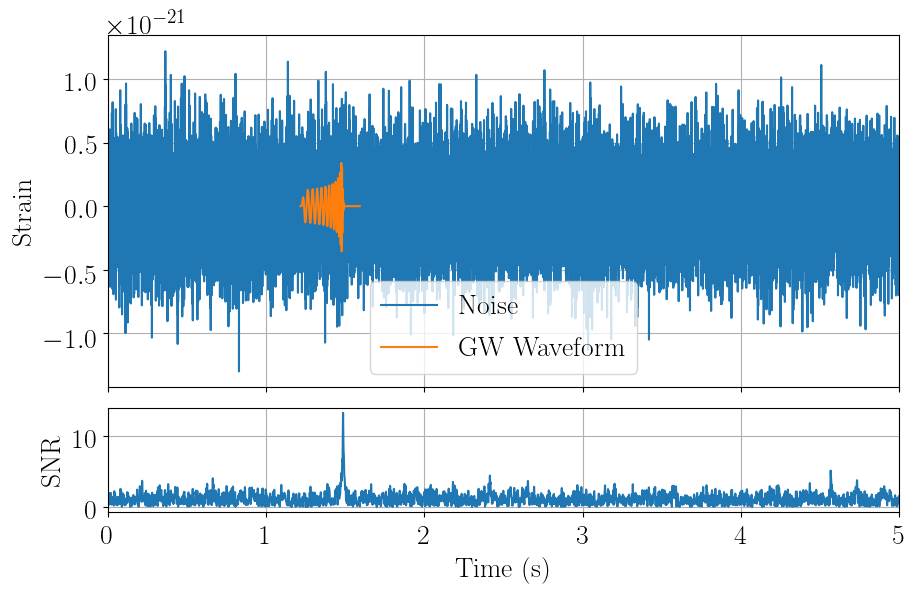
\includegraphics[width=\columnwidth]{snr3.png} 
   \caption{A schematic illustration for the match-filtering. In the above figure a $30M_\odot-30M_\odot$ \ac{BBH} signal from a luminosity distance of $2000$ Mpc is injected into the colored Gaussian noise generated from the designed sensitivity of Advanced LIGO. The lower figure shows the match-filtering \ac{SNR} using the same signal as a template.}
   \label{fig:snr}
\end{figure}


\subsection{Parameter Estimation}\label{subsec:pe}

Once a \ac{GW} signal is triggered by the search pipeline and confirmed to be a detection, we can proceed to the parameter estimation stage.
The Bayesian inference lays the foundation of the framework of parameter estimation (see e.g. \cite{sivia2006data}).
The Bayesian framework is particular useful when we have a deterministic model which can be used to make a direct comparison with the data \cite{bayesintro}.

The Bayesian theorem claims
\be\label{eq:bayesformula}
P(A|B) = \frac{P(B|A)P(A)}{P(B)}
\ee
where $A$ and $B$ are random events associated with a probability distribution.

In the context of \ac{GW} parameter estimation, one can substantiate the events in \cref{eq:bayesformula} by ``Detection of \ac{GW} strain $d$'' and ``The data can be predicted by the model $H$ with parameters $\vec{\theta}$''
\be\label{eq:pe}
P(\vec{\theta}|d,H,I) = \frac{ P(d|\vec{\theta},H,I) P(\vec{\theta}|H,I)} {P(d|H,I)}.
\ee
For example, $H$ can be the hypothesis that the \ac{GW} data $d$ contains a \ac{GW} signal from the coalescence of a pair of \ac{BH} with parameters $\vec\theta$, $I$ is any other background information, such as assuming that \ac{GR} is correct.

\cref{eq:pe} is the essential formula for \ac{GW} parameter estimation. 
$P(\vec{\theta}|H,I)$ is the prior distribution for $\vec{\theta}$, representing the knowledge about the range of parameter values before starting measurements. 
The likelihood function $P(d|\vec{\theta},H,I)$ gives the possibility of obtaining the data from a specific set of model parameters.
The posterior $P(\vec{\theta}|d,H,I)$ contained all the information about the results of parameter estimation.
It is used to make a quantitative statement about the parameters, such as median value and error bar.

In the context of \ac{GW} data analysis, for an ideal case, the detector noise is assumed to be Gaussian and stationary, therefore the likelihood function is
\be \label{eq:likelihood}
P(d|\vec{\theta}, H, I) \propto \exp\[	-\frac{1}{2} \(d-h(\vec{\theta})|d-h(\vec{\theta})\)\]
\ee
where $h(\vec{\theta})$ is the \ac{GW} template.
\cref{eq:likelihood} is a generalization of the one-dimensional Gaussian distribution to infinite dimensions in frequency space.
Due to the lack of an analytical results and a high computational complexity caused by the large parameter dimensions, the sampling of the likelihood function is done by Markov Chain Monte Carlo or Nested Sampling \cite{lalinference,skilling2004nested}.

Furthermore, the one-dimensional distribution for a specific parameter $\theta_1 \in \vec\theta$ can be obtained by marginalizing other parameters  
\be \label{eq:onedimpe}
P(\theta_1|d,H,I) = \int d\theta_2 d\theta_3 ... d\theta_N P(\vec{\theta}|d,H,I).
\ee
The resulting distribution of \Cref{eq:onedimpe} from observation is used to announce the information of a \ac{GW} event, e.g., ``The chirp mass of the \ac{GW} event GW150914 from \ac{BBH} merger is $28.6^{+1.6}_{-1.5} M_\odot$ ($90\%$ confidence interval)'' actually means that the median value of the distribution $P(\mathcal{M}_c|d,H,I)$ is $28.6 M_\odot$ and the $90\%$ confidence interval is $[28.6-1.5, 28.6+1.6] M_\odot$.
The model of \ac{BBH} with quasi-circular obit coalescence has 15 degree of freedoms for source parameters: two masses, two spin vectors each having three components, the coalescence time and phase, the inclination and polarization angle, the position in the three dimensional space.

Another theme of Bayesian statistics is model selection which is to select the best model favored by observation.
Normalizing both sides of \cref{eq:pe}, the evidence can be obtained as a constant given the data $d$
\be 
P(d|H,I) = \int d\vec{\theta} P(d|\vec{\theta},H,I) P(\vec{\theta}|H,I).
\ee
The so-called Bayesian ratio is defined as the ratio of evidence of two competitive models $H_1$ and $H_2$, e.g., \ac{GR} and modified gravity model beyond \ac{GR},
\be 
\mathcal{B}^1_2 = \frac{P(d|H_1,I)}{P(d|H_2,I)}.
\ee
Making use of the Bayesian formula \cref{eq:bayesformula} again, we obtain
\be 
P(H|d,I) = \frac{P(d|H,I)P(H|I)}{P(d|I)}.
\ee
The odds ratio between model $H_1$ and model $H_2$ can be expressed by
\be \label{eq:oddsratio}
\mathcal{O}^1_2 = \frac{P(H_1|d,I)}{P(H_2|d,I} = \frac{P(d|H_1,I)}{P(d|H_2,I)} \frac{P(H_1|I)}{P(H_2|I)} = \mathcal{B}^1_2 \frac{P(H_1|I)}{P(H_2|I)}.
\ee
The odds ratio reflects quantitatively which model is favored by data from observation.
From \cref{eq:oddsratio}, we can see that the odds ratio differs from the Bayesian ratio by a factor related to the prior of models.
If the competitive models are assumed to be equally likely before any measurement, then odds ratio is equal to Bayesian ratio. 

%%%%%%%%%%%%%%%%%%%%%%%%%%%%%%%%%%%%%%%%%%%



\chapterend

\chapter{Overview of Stochastic Gravitational-Wave Background}\label{ch:SGWBOverview}

\section{Mathematical Characteristics}

The first part of the thesis have discussed detection and implications of \acp{GW} from individual \ac{CBC} events which are loud enough to pass the detection threshold.
There also exists an incoherent superposition from numerous \acp{GW} which can not be resolved individually, including those too weak to be detected or having intrinsic stochastic nature, for example, the primordial \ac{GW} is generated by random quantum fluctuations in the early Universe.
\ac{SGWB} is another important type of \ac{GW} that LIGO and Virgo are searching for.
The data analysis techniques used for \ac{SGWB} is different from those for searching for \ac{CBC} signals in the sense that there are no deterministic waveform templates.
The search for \ac{SGWB} relies on the cross correlation technique which will be discussed in the following section.
In this section we define the basic quantities to characterize \ac{SGWB}.

Due to the stochastic nature, \ac{SGWB} is characterized by its statistical properties. 
The dimensionless fractional energy density spectrum is usually used to describe the intensity of \ac{SGWB}, which is defined as
\be
\Omega_\text{GW}(f) \equiv \frac{f}{\rho_c}\frac{d\rho_\text{GW}}{d f} 
\ee
where $d\rho_\text{GW}$ is the \ac{GW} energy density in the frequency range $[f,f+df]$, $\rho_c = 3H_0^2c^2/(8\pi G)$ is the critical energy density needed for a close Universe, $H_0$ is the value of Hubble constant of today.

We next follow Refs.~\cite{SGWBseminal1,SGWBseminal2,SGWBlivingreview} to briefly derive the relation between $\Omega_\text{GW}$ and \ac{GW} metric tensor $h_{\mu\nu}$ obtained from the weak field approximation as described in \cref{ch:review1}.
Qualitatively the \ac{GW} energy density at a specific space point is proportional to the square of \ac{GW} strain.
In the transverse traceless gauge, the plane wave expansion for \ac{GW} emitted from a given direction can be written as
\be\label{eq:hijplanewave}
h_{ij}^{TT}(t,\vec{x}) = \sum_A \int df \int_{S^2} d{\Omega}_{\hat{n}}~ h_A(f,\hat{n})e^A_{ij}(\hat{n}) e^{i 2\pi f (t- \hat{n}\cdot\vec{x}/c)}
\ee
where $\hat{n}$ is the unit vector pointing to the direction of \ac{GW} propagation, ${\Omega}_{\hat{n}}$ is the solid angle of the two-sphere associated with $\hat{n}$, $A =\{+,\times\}$ denotes the plus and cross polarization patterns, $h_A(f,\hat{n}) = \{h_+(f,\hat{n}),h_\times(f,\hat{n})\}$ are the Fourier components of \acp{GW}, $e^A_{ij}(\hat{n}) = \{e^+_{ij}(\hat{n}),e^\times_{ij}(\hat{n})\}$ are the bases of plus and cross polarization.

Assuming the \ac{SGWB} under consideration is stationary, isotropic, Gaussian and non-polarized, the \ac{GW} strain \ac{PSD} $S_h(f)$ can be defined as the ensemble expectation of the quadratic of \ac{GW} Fourier components
\be \label{eq:have}
\< h_A(f,\hat{n}) h_{A'}^\ast(f',\hat{n'}) \> = \frac{1}{16\pi} S_h(f) \delta(f-f') \delta_{AA'} \delta^2({\Omega}_{\hat{n}}-{\Omega}_{\hat{n}'}).
\ee
The superscript $\ast$ denotes the complex conjugate.
The last three Delta functions in the above expression corresponds to the assumption of stationary, unpolarized and isotropic background, respectively.

The \ac{GW} stress-energy tensor can be obtained by averaging over a few wave cycles where the spatial size is larger than the wavelength of \acp{GW} but smaller than the arm-length of detectors. 
Effectively, this is a procedure to separate \acp{GW} from background.
The mathematical expression can be found, e.g., in Eq.~(1.133) of Ref.~\cite{maggiore2008gravitational}
\be 
T^\text{GW}_{\mu\nu} = \frac{c^4}{32\pi G}\< h_{\alpha\beta,\mu}h^{\alpha\beta}_{~~,\nu}\>.
\ee
The energy density $\rho_\text{GW}$ is the $(0,0)$ component of $T^\text{GW}_{\mu\nu}$.
Choosing the transverse and traceless gauge, the expression is
\be\label{eq:rhogw}
\rho_\text{GW} =  T_{00}^{\text{GW}} = \frac{c^2}{32\pi G}\<\dot{h_{ij}}(t,\vec{x})_\textrm{TT}~ \dot{h^{ij}}(t,\vec{x})_\textrm{TT}\>
\ee
where the upper dot denotes the derivative with respect to time.
Substituing \cref{eq:hijplanewave} and \cref{eq:have} into \cref{eq:rhogw} yields
\begin{align}\label{eq:rhogwandshf}
\rho_\text{GW} =& \frac{c^2}{32\pi G}\int df df' d{\Omega} d{\Omega'} (2\pi i f)(-2\pi i f') 
\<h_A(f,\hat{n})h_{A'}^\ast(f',\hat{n'})\>e_{ij}^Ae^{ij}_{A'} \times\nn\\ 
&\exp\[2\pi i f\(t-\frac{\hat{n}\cdot \vec{x}}{c}\)\]
\exp\[-2\pi i f' \(t-\frac{\hat{n'}\cdot \vec{x}}{c}\)\] \nn\\
=&\frac{\pi c^2}{4G} \int_0^\infty df f^2 S_h(f)
\end{align}
For a concise expression we have neglected the subscript ``TT'' for \ac{GW}.
In deriving the above result we have used the following relation
\be
\int d{\Omega} = 4\pi, ~e_{ij}^+ e^{ij}_+=2~\textrm{and}~e_{ij}^\times e^{ij}_\times=2.
\ee
Since
\be\label{eq:rhogwdif}
\rho_\text{GW} = \int_0^\infty \frac{d\rho_\text{GW}}{df} df,
\ee
comparing \cref{eq:rhogwdif} with Eq.~(\ref{eq:rhogwandshf}) yields
\be 
\frac{d\rho_\text{GW}}{df} = \frac{\pi c^2}{4G} f^2 S_h(f),
\ee
therefore
\be 
\Omega_\text{GW}(f) = \frac{2\pi^2 f^3}{3H_0^2} S_h(f).
\ee
This is the relation between $\Omega_\text{GW}(f)$ and the one-sided \ac{PSD} of \ac{GW} strain.

Another useful quantity is the characteristic strain of \acp{GW} which is defined as
\be 
h_c(f) \equiv \sqrt{fS_h(f)}.
\ee
It is straightforward to obtain
\be 
\Omega_\text{GW}(f) = \frac{2\pi^2}{3H_0^2} f^2 h_c^2(f).
\ee

In \cref{fig:characteristic-strain}, we show examples of \ac{GW} and noise characteristic strains.
The noise is generated using the \texttt{aLIGOZeroDetHighPower} (standing for ``Advanced LIGO Zero Detuned High Power'') \ac{PSD} model from the {\PYCBC} package \cite{pycbc}. 
The \ac{GW} characteristic strains are generated using the plus polarization pattern of {\IMRP} model from $10-10~M_\odot$ and $30-30~M_\odot$ \ac{BBH} merger, respectively. 
The source distance is set to be $1$ Gpc.

\begin{figure}[htbp]
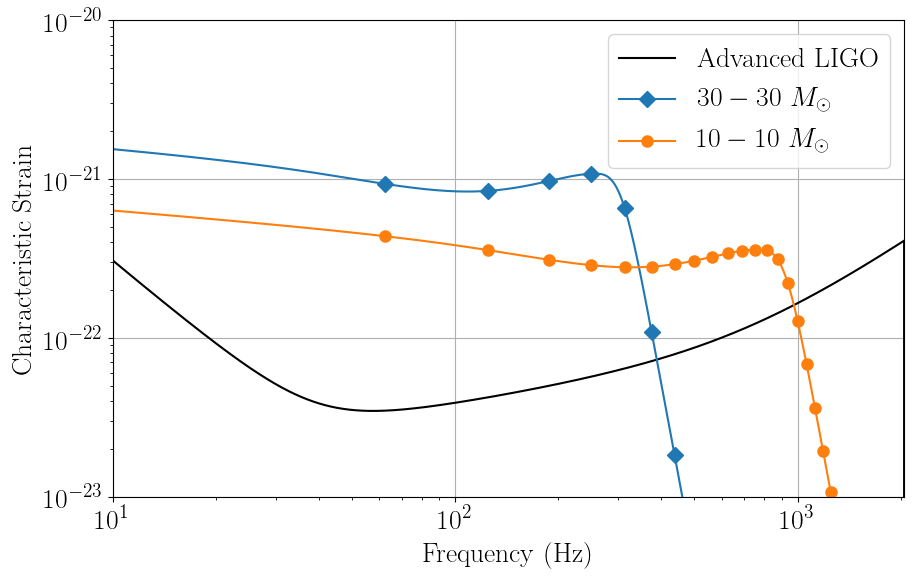
\includegraphics[width=\columnwidth]{character.png}
  \caption{Examples of \ac{GW} and noise characteristic strains.
The noise is from the \texttt{aLIGOZeroDetHighPower} \ac{PSD} model.
The \ac{GW} characteristic strains are generated using the plus polarization pattern of {\IMRP} model from $10-10~M_\odot$ and $30-30~M_\odot$ \ac{BBH} merger, respectively. 
The source distance is $1$ Gpc.}
  \label{fig:characteristic-strain}
\end{figure}

We also derive the \ac{GW} differential energy with respect to frequency, $dE/df$, which will be used to derive an explicit expression for $\Omega_\text{GW}$ in the next section.
Integrating both sides of \cref{eq:have} with respect to solid angle, one obtains
\be 
\< h_A(f) h_{A'}^\ast(f') \> = \int d\Omega_{\hat{n}} d\Omega_{\hat{n}'} \< h_A(f,\hat{n}) h_{A'}^\ast(f',\hat{n'}) \> = \frac{1}{4} S_h(f) \delta(f-f') \delta_{AA'} .
\ee
Let $A=A'$ and $f=f'$, one gets
\be \label{eq:shoff-and-delta}
\< |h_+(f)|^2\>  =\< |h_\times (f)|^2\>  = \frac{1}{4} S_h(f) \delta(0).
\ee
The energy density $\rho_\text{GW}$ is related to $dE$ by
\be 
\frac{d^2E}{dA cdt} = \rho_\text{GW} = \frac{\pi c^2}{4G}\int_0^\infty df f^2 S_h(f) 
\ee
where $dA$ is the differential area, therefore
\be \label{eq:deoverda}
\frac{dE}{dA} = \frac{\pi c^3}{4G}\int_0^\infty df ~f^2 S_h(f)~\int_{-\infty}^\infty dt 
\ee
Because $\delta(f) = \int_{-\infty}^\infty \exp[2\pi i f t] dt $, we substitute $\delta(0) = \int_{-\infty}^\infty dt $ and \cref{eq:shoff-and-delta} into \cref{eq:deoverda}
\be 
\frac{dE}{dA} = \frac{\pi c^3}{4G}\int_0^\infty df  f^2 S_h(f) \delta(0) = \frac{\pi c^3}{G}\int_0^\infty df f^2  \< |h_+(f)|^2\>
\ee
If $h_A(f)$ has a deterministic form without any intrinsic randomness and the observation time is long enough compared with the duration of \ac{GW} transient signals, the ensemble bracket of $h(f)$ can be removed, therefore
\be \label{eq:dEoverdf-to-hplus}
\frac{dE}{df} = \frac{\pi c^3}{G} f^2  d_L^2  \int d\Omega |h_+(f)|^2 = \frac{4\pi^2 c^3}{G}f^2 d_L^2 |h_+(f)|^2,
\ee
where $d_L$ is the luminosity distance to the source.

\section{$\Omega_\text{GW}(f)$ from Binary Black Hole Coalescence}

Many different \ac{GW} emission mechanisms can give rise to \ac{SGWB} in the ground-based \ac{GW} detector frequency band ($\sim[10,10^3]$ Hz), to name a few, stellar mass \ac{CBC}, core collapse supernovae and burst of cosmic strings \cite{Christensen:sgwbreview}.
So far all detected \ac{GW} events come from the coalescence of \ac{BBH} and \ac{BNS}, thus allowing us to infer the event rate, especially the lower limit of the event rate.
The amplitude of \ac{SGWB} spectrum arising from \ac{CBC} is totally determined by the event rate. 
Other modeling systematics of compact binary population synthesis only contribute the next-to-leading order of amplitude.
According to the event rate inference, \ac{SGWB} from \ac{CBC} have a chance to be detected with the designed sensitivity of Advanced LIGO and Virgo around the year of 2020 to 2022 \cite{TheLIGOScientific:2016wyq,TheLIGOScientific:2016dpb,Abbott:2017xzg,LIGO-sgwb-o2-iso}.

Next we derive the expression for $\Omega_\text{GW}(f)$ contributed by \ac{BBH} merger of astrophysical origin, as opposed to the \acp{BH} of primordial origin which will be discussed in detail in the next chapter.

It is convenient to start from the \ac{GW} flux, which is related to the energy density $\rho_\text{GW}$ by 
\begin{equation}\label{eq:drhodnu}
\frac{d\rho_{GW}}{df}=\frac{F(f)}{c}.
\end{equation}
Here $F(f)$ is the energy flux in the frequency range $[f,f+df]$.

Schematically, the contribution to flux $F(f)$ should be an integral over all the \ac{BBH} sources in the Universe,
\be
F(f)=\int_{\textrm{space}} \textrm{BBH number density} \times \textrm{Flux from a BBH}\times dV
\ee
where $dV$ is the infinitesimal volume element.
At a specific moment, the \ac{SGWB} received by a detector should have been emitted earlier because \acp{GW} travel at a finite speed $c$.
Therefore, integrating with respect to space volume from near to far is equivalent to integrating with respect to cosmic time, or equivalently, cosmological redshift $z$ \cite{Rosado:2011kv}.
The above description can be expressed quantitatively by
\begin{equation}\label{eq:flux}
F(f)=\int_{z_{inf}}^{z_{sup}} \frac{1}{4\pi d_L^2(z)}\frac{dE_\text{GW}(f)}{df} R_z(z)dz
\end{equation}
where $R_z(z)dz$ is the number density rate of \ac{BBH} merger events in the redshift interval $[z,z+dz]$ as observed in the detector (Earth) frame, $dE_\text{GW}(f)/{df}$ is the spectral \ac{GW} energy emitted by a single \ac{BBH} merger in the detector frame, $d_L(z) = (1+z) r(z)$ is the luminosity distance, $r(z)$ is the proper distance to the source.

Therefore we can derive a formal expression for the \ac{SGWB} energy density spectrum from \ac{BBH} \ac{CBC}
\begin{align}
\Omega_{\textrm{GW}}(f) = \frac{f}{\rho_\textrm{c}H_0} \int_{0}^{z_{\textrm{sup}}} \frac{R_z(z)}{(1+z)E(z)} \times   \frac{dE}{df_\textrm{s}}(f_\textrm{s}) \, dz,
\end{align}

Usually $R_z(z)$ can be converted to the mass density rate of binary star coalescence $R_V(z)$ in the comoving volume interval $[V_c,V_c+dV_c]$ by the following expression \cite{SGWB-sfr-relation-1,Wu:2011ac}
\begin{equation}\label{eq:rzsfr}
R_z(z)=\lambda R_V(z)\frac {dV_c(z)}{dz}~,
\end{equation}
where  $\lambda$ is a constant describing the mass fraction of \acp{BBH} in binary coalescence in unit of $M_\odot^{-1}$, $dV_c(z)$ is the infinitesimal comoving volume element. 
The mass density rate $R_V(z)$ follows in turn the astrophysical star formation rate $R_\ast$.
There is a time delay $t_d$ from the star formation to the coalescence of binaries, therefore, $R_V(z)$ can be expressed by the following convolution
\begin{equation}\label{eq:sfr}
R_V(z)=\int \frac{1}{1+z_f} R_\ast(t_c'(z)-t_d)P(t_d)dt_d~,
\end{equation}
where $R_\ast$ is in unit of mass per unit time per unit comoving volume, $t_c'$ is the cosmic time for binary coalescence, $z_f$ is the redshift corresponding to cosmic time $t_c'(z)-t_d$.
The constant $\lambda R_V(z=0)$ corresponds to the local merger rate of \ac{BBH} coalescence, which is estimated to be $ 53.2_{-28.8}^{+58.5}~ \text{Gpc}^{-3} \text{yr}^{-1}$ after the second observation run of Advanced LIGO and Virgo \cite{GWTC1-rate}.
The factor $1+z_f$ in the denominator accounts for the time dilation due to the cosmic expansion, converting the star formation rate from the source frame to the detector frame.
A common parametrization for the probability distribution of time delay is of the power law form, i.e., $P(t_d)\sim t_d^\alpha$, while $\alpha=1$ is preferred.
An example of the star formation rate parametrization is the Beacom and Hopkins model \cite{sfr-Hopkins_2006} with the following form
\begin{equation}
R_*(z)=h_0\frac{0.017+0.13z}{1+(z/3.3)^{5.3}} M_\odot,
\end{equation}
the unit is $M_\odot ~\text{yr}^{-1}~ \text{Mpc}^{-3}$, $h_0$ is the value of Hubble parameter of today in unit of $100$ km/s/Mpc, i.e., $H_0 = 100h_0$.

Before proceeding we derive some equalities in the context of an expanding flat Universe which will be used to further simplify \cref{eq:flux} \cite{Rosado:2011kv}.
The \ac{FLRW} metric describing the flat Universe in expansion is
\be\label{eq:FRW}
ds^2 = -c^2 dt^2 +a^2(t)(dr^2 + d\Omega^2 )
\ee
where one should note that $t$ is the cosmic looking back time, $a(t)$ is the scale factor and $(r,\Omega)$ is a set of comoving spherical coordinate.
The cosmological redshift $z$ has the following relation with $a(t)$
\be\label{eq:redshift}
1+z = \frac{a(0)}{a(t)}.
\ee
Conventionally the scale factor of today is set to unity, i.e., $a(0) = 1$. 

The proper time of light is zero, leading to $ds^2 = 0$, therefore
\be 
dr = \frac{c}{a(t)}dt
\ee
while $d\Omega =0$ is chosen by considering the direction of line of sight. 
By differentiating \cref{eq:redshift} and substituting the expression for Hubble parameter $H(z) = - \dot{a}/a$, one obtains
\be 
dt = \frac{1}{(1+z)H(z)} dz 
\ee
The differential comoving volume is given by
\be 
dV_c = 4\pi r^2 dr
\ee
therefore 
\begin{equation}\label{eq:dvdz}
dV_c(z)=\frac{4\pi c}{H_0} \frac{r^2(z)}{\sqrt {\Omega_M(1+z)^3+\Omega_\Lambda}}dz
\end{equation}
where
\be 
H(z) = H_0 \sqrt{\Omega_M(1+z)^3 + \Omega_\Lambda},
\ee
$\Omega_M$ and $\Omega_\Lambda$ are the fraction of the energy density of matter and dark energy to the total energy density in the Universe, respectively.

There remains another term which has not been discussed,  the \ac{GW} differential energy $dE/df$ in the frequency domain.
For calculating the \ac{SGWB} energy density spectrum from \ac{BBH} coalescence, we use the aligned-spinning \ac{BBH} tempalte {\IMRB} due to its relatively simple parametrization.
Substituting the expression of \cref{eq:templatestrain} into \cref{eq:dEoverdf-to-hplus}, we get
\be \label{eq:dEoverdf-final}
\frac{dE}{df} = \frac{(G\pi)^{2/3} M_c^{5/3}}{3}f^2 f_1^{-7/3} 
\left\{ 
\begin{aligned}
& \[ f'^{-7/6}\(1+\sum_{i=2}^{3}\alpha_i v^i\) \]^2, &\mathrm{if}~ f< f_1\\ 
& \[ w_m f'^{-2/3} \(1+ \sum_{i=1}^{2} \epsilon_i v^i\) \]^2, &\mathrm{if} ~f_1 \leq f < f_2\\
& \[ w_r \mathcal{L}(f,f_2,\sigma) \]^2,                    &\mathrm{if} ~f_2 \leq f < f_3
\end{aligned} 
\right. 
\ee 
Note that we have multiplied $h_+(f)$ by a factor of $\sqrt{2/5}$ \cite{maggiore2008gravitational} to take into account the average effect of sources from all-sky.
One should note that when considering a \ac{BBH} source at redshift $z$, the chirp mass in \cref{eq:dEoverdf-final} should be substitute by the redshifted chirp mass $M_c^z=(1+z)M_c$, and the source frequency $f_s = (1+z) f$ should be used instead of the detector frequency $f$.
This is accounted by the propagation of \ac{GW} in an expanding Universe.

If we only consider the inspiral part of the \ac{CBC} signal using the quadripolar approximation, as is the case for calculating \ac{SGWB} from \ac{BNS}, the \ac{GW} energy spectrum at redshift z is given by
\be\label{eq:dednu}
\frac{dE}{df_s}=\frac{(G\pi)^3}{3}(M_c^z)^{5/3}f_s^{-1/3}~,
\ee
Substituting \cref{eq:dednu,eq:rzsfr,eq:sfr,eq:dvdz} into \cref{eq:flux,eq:drhodnu}, one obtains the analytical expression for \ac{SGWB} from \ac{BNS} coalescence
\begin{equation}\label{eq:BNSSGWB}
\Omega_{GW}(f)=\frac{8\lambda (\pi GM_c)^{5/3}}{9H_0^3 c^2}f^{2/3}\int ^{z_{\textrm{sup}}}_0\frac{R_V(z)dz}{(1+z)^{1/3}{\sqrt {\Omega_M(1+z)^3+\Omega_\Lambda}}}~,
\end{equation}
where$z_\text{sup}=$
$
\centering
\begin{cases}
z_{max}, &\textrm{if}~f<f_\textrm{max}/(1+z_\textrm{max}) \\
{f_\textrm{max}}/{f}-1,~&\textrm{otherwise}
\end{cases}
$,  
$z_\text{max}$ and $f_\text{max}$ are the maximum cutoff for redshift and frequency.
The parameter $\lambda$ describing the mass fraction of \ac{BNS} in binary coalescence in \cref{eq:BNSSGWB} should be obtained from corresponding population synthesis analysis.

\section{Searching for Isotropic Stochastic Background}

We proceed to discuss the data analysis technique used for searching for an isotropic \ac{SGWB}.
Due to its stochastic nature, the signal of \ac{SGWB} just acts as Gaussian random noise.
Therefore, the essential idea is to utilize correlation analysis between multiple \ac{GW} detectors to identify a correlated background signal, while the noise arising from environments are uncorrelated.
We follow the seminal paper Ref.~\cite{SGWBseminal1,SGWBseminal2} to set up the relevant data analysis framework for isotropic \ac{SGWB} searches.

Assuming there are two separated detectors, as is the case for Advanced LIGO, the detectors' output $s_i(t)$ can be expressed by
\be 
s_i(t) = h_i(t) + n_i(t), ~(i=1,2)
\ee
where $h_i(t)$ and $n_i(t)$ are \acp{GW} and noise, respectively.
One can obtain the following cross correlation statistics of signal
\be 
S = \int_{-T/2}^{T/2}dt\int_{-T/2}^{T/2}dt' s_1(t) s_2(t')Q(t,t')
\ee
where $T$ is the time duration of observation, $Q(t,t')$ is the filter to be determined by maximizing the \ac{SNR}.
If the \ac{GW} background and noise are both stationary, then $Q(t,t') = Q(t-t')$ and the filter only depends on the time difference.

Using the Fourier transformation
\begin{eqnarray}
s_i(t) &=& \int_{-\infty}^{\infty} \tilde{s_i}(f) e^{2\pi i f t} df \nn \\
Q(t-t')&=&  \int_{-\infty}^{\infty} \tilde{Q}(f'') e^{2\pi i f'' (t-t')} df''
\end{eqnarray}
One obtains
\begin{eqnarray} \label{eq:sgwbsignal}
S &=& \int_{-T/2}^{T/2}dt \int_{-T/2}^{T/2}dt' \int_{-\infty}^{\infty} df \int_{-\infty}^{\infty} df' \int_{-\infty}^{\infty} df'' \tilde{s_1}^\ast (f) \tilde{s_2}(f') \tilde{Q}(f'') \times \nn\\
&& \exp{\[2\pi i (f''-f)t\]}\exp{\[2\pi i (f'-f'')t'\]} \nn\\
&=& \int_{-\infty}^{\infty} df df' df'' \delta_T(f''-f) \delta_T(f'-f'') \tilde{s_1}^\ast(f) \tilde{s_2}(f') \tilde{Q}(f'') \nn \\
&\approx & \int_{-\infty}^{\infty} \tilde{s_1}^\ast(f) \tilde{s_2}(f) \tilde{Q}(f) df 
\end{eqnarray}
where $\delta_T(f)$ is the Dirac Delta function in the finite time limit 
\be 
\delta_T(f) \equiv \int_{-T/2}^{T/2} e^{2\pi i ft} dt = \frac{\sin (\pi f T)}{\pi f}
\ee
The last line of Eq.~(\ref{eq:sgwbsignal}) is justified in the limit of large $fT$ which leads to $\delta_T(f) \approx \delta(f)$.

In the context of \ac{SGWB}, the \ac{SNR} is defined as the ratio of the expectation value of $S$ and the standard variance of $S$.
The expectation can be expressed by
\begin{eqnarray}\label{eq:means}
\< S \> &=& \int_{-\infty}^{\infty} \< \tilde{s_1}^\ast(f) \tilde{s_2}(f) \> \tilde{Q}(f) df \nn\\  
&=& \int_{-\infty}^{\infty} \< \tilde{h_1}^\ast(f) \tilde{h_2}(f) \> \tilde{Q}(f) df.
\end{eqnarray}
The second line of the above is obtained since the mean value of noise is zero.

We again write down the plane wave expansion for $\tilde{h_i}(f)$, but here is the \ac{GW} strain received by the detector which have taken the beam pattern function into account.
The following equality is obtained by multiplying \cref{eq:hijplanewave} by the detector tensor $D^{ij}$
\be 
h_i(t,\vec{x}_i) = \sum_{A=+,\times}\int_{-\infty}^{\infty} df \int d\hat{\Omega}_{\hat{n}} \tilde{h_A}(f,\hat{n})e ^{2\pi i f(t-\hat{n}\cdot \vec{x_i}/c) }F_i^A(\hat{n})
\ee
where $F_i^A(\hat{n})$ is the beam pattern function of the $i$-th detector.
The Fourier transformation of the above \ac{GW} strain is
\be \label{eq:tildehi}
\tilde{h_i}(f) = \sum_{A=+,\times} \int d\hat{\Omega}_{\hat{n}} \hat{h}_A(f) (f,\hat{n}) e^{-2\pi i f\hat{n}\cdot \vec{x_i}/c} F_i^A(\hat{n})
\ee
Substituting \cref{eq:tildehi} into Eq.~(\ref{eq:means}), one obtains
\begin{eqnarray}\label{eq:means2}
\< S \> &=& \int_{-\infty}^{\infty} df \< \tilde{h}_1^\ast(f) \tilde{h}_2(f)\>\tilde{Q}(f)\nn \\
&=&  \int_{-\infty}^{\infty}df \sum_{A,A'} \int d\hat{\Omega}_{\hat{n}} d\hat{\Omega}_{\hat{n'}} \<h_A^\ast(f,\hat{n}) h_{A'}(f,\hat{n'}) \> e^{2\pi i f\hat{n}\cdot \vec{x_1}/c}e^{-2\pi i f'\hat{n'}\cdot\vec{x_2}/c} F_1^A(\hat{n}) F_2^{A'}(\hat{n'}) \tilde{Q}(f)\nn \\
&=&  \int_{-\infty}^{\infty}df \sum_{A,A'} \int d\hat{\Omega}_{\hat{n}} d\hat{\Omega}_{\hat{n'}} \frac{1}{16\pi}S_h(f) \delta(f-f)\delta_{AA'}\delta(\hat{\Omega}_{\hat{n}}-\hat{\Omega}_{\hat{n'}}) \nn\\
&&\times e^{2\pi i f\hat{n}\cdot \vec{x_1}/c}e^{-2\pi i f'\hat{n'}\cdot\vec{x_2}/c} F_1^A(\hat{n}) F_2^{A'}(\hat{n'})\tilde{Q}(f) \nn \\
&=& \int_{-\infty}^{\infty} df \delta(0) \frac{1}{16\pi} S_h(f) \sum_A\int d\hat{\Omega}_{\hat{n}} e^{2\pi i f \hat{n}\cdot \Delta\vec{x}/c}F_1^A(\hat{n}) F_2^A(\hat{n}) \tilde{Q}(f)
\end{eqnarray}
where $\Delta\vec{x} =\vec{x}_1-\vec{x}_2$.

For a pair of \ac{GW} detectors, the overlap reduction function $\gamma(f)$ is defined as follows
\be 
\gamma(f) \equiv \frac{5}{8\pi} \sum_A \int d \hat{\Omega}_{\hat{n}} e^{2\pi i f\vec{n}\cdot\Delta\vec{x}/c} F_1^A(\hat{n})F_2^A(\hat{n'})
\ee
where $\vec{\delta x}$ is the separation vector between the central positions of the two detectors.
The overlap reduction function describes the degree of reduction of coherent \ac{GW} signal due to the non-parallel alignment and the geographical separation of the two detectors. 

The Eq.~(\ref{eq:means2}) can be expressed by $\gamma(f)$ and $\Omega_\text{GW}(f)$ by
\begin{eqnarray}
\<S\> &=& \int_{-\infty}^{\infty} df \delta(0) \frac{1}{16\pi} S_h(f) \frac{8\pi}{5}\gamma(f) \tilde{Q}(f)\nn\\
&=& \frac{3H_0^2}{20\pi^2} T \int_{-\infty}^{\infty}df |f|^{-3}\Omega_\text{GW}(|f|)\gamma(f)\tilde{Q}(f)
\end{eqnarray}
where the term $T$ arises from the finite time approximation of $\delta(0)$, i.e., $\delta(0) = \int_{-T/2}^{T/2}dt = T$, the absolute value of $f$ is due to the fact that $S_h(f)$ is defined as the one-sided \ac{GW} \ac{PSD}.

We continue to derive the variance of $S$
\begin{eqnarray}\label{eq:svariance}
\sigma^2 \equiv\[ \<S^2\> -\<S\>^2\]_{h=0} &=& \int_{-\infty}^{\infty} df df'\tilde{Q}(f)\tilde{Q}^\ast(f')\times\nn\\
&&\[\<\tilde{n}_1^\ast(f)\tilde{n}_2(f) \tilde{n}_1^\ast(f') \tilde{n}_2(f')\> - \< \tilde{n}_1^\ast(f)\tilde{n}_2(f)\> \< \tilde{n}_1^\ast(f') \tilde{n}_2(f')\>\]\nn\\
&=&\int_{-\infty}^{\infty} df df'\tilde{Q}(f)\tilde{Q}^\ast(f')\<\tilde{n}_1^\ast(f)\tilde{n}_2(f) \tilde{n}_1^\ast(f') \tilde{n}_2(f')\>
\end{eqnarray}
The second line is obtained due to the assumption that the noise between two detectors has no correlation.
This assumption also reduces Eq.~(\ref{eq:svariance}) to
\be 
\sigma^2 =\int_{-\infty}^{\infty} df df'\tilde{Q}(f)\tilde{Q}^\ast(f')\<\tilde{n}_1^\ast(f)\tilde{n}_2(f)\>\< \tilde{n}_1^\ast(f') \tilde{n}_2(f')\>.
\ee
We write down again the definition of noise \ac{PSD}
\be 
\<\tilde{n}^\ast(f)\tilde{n}(f')\> =\frac{1}{2} \delta(f-f') P(f),
\ee
therefore
\be 
\sigma^2 = \frac{T}{4} \int_{-\infty}^{\infty} df P_1(|f|) P_2(|f|) |\tilde{Q}(f)|^2.
\ee
Again we have used the finite time approximation for $\delta(0)$ and the absolute value of frequency is because $P(f)$ is the one-sided noise \ac{PSD}.

It is convenient to define the inner product of the following form
\be 
(A,B) \equiv \int_{-\infty}^{\infty} df A^\ast(f) B(f) P_1(|f|)P_2(|f|).
\ee
where $A(f)$ and $B(f)$ are arbitrary functions.
The mean value and variance of $S$ can be expressed in terms of this inner product by
\be 
\<S\> = \frac{3H_0}{20\pi^2} T\(\tilde{Q},\frac{\gamma(f)\Omega_\text{GW}(|f|)}{|f|^3P_1(|f|)P_2(|f|)}\),
\ee
and
\be 
\sigma^2= \frac{T}{4}\(\tilde{Q},\tilde{Q}\).
\ee
The square of \ac{SNR} for \ac{SGWB} searches can be defined by
\be 
\textrm{SNR}^2 = \frac{\<S\>^2}{\sigma^2} = \( \frac{3H_0^2}{10\pi^2}\)^2T\frac{\(\tilde{Q},\frac{\gamma(f)\Omega_\text{GW}(|f|)}{|f|^3P_1(|f|)P_2(|f|)}\)}{\(\tilde{Q},\tilde{Q}\)}.
\ee
To maximize the \ac{SNR}, the optimal filter $\tilde{Q}(f)$ should be chosen as
\be 
\tilde{Q}(f) =\mathcal{N}\frac{\gamma(f)\Omega_\text{GW}(|f|)}{|f|^3P_1(|f|)P_2(|f|)}.
\ee
Usually the energy density spectrum of \ac{SGWB} takes the power law form, i.e., $\Omega_\text{GW}(f) = \Omega_\alpha(f/f_\textrm{ref})^\alpha$.
The normalization factor of the optimal filter $\mathcal{N}$ is so determined that $\<S\> = \Omega_\alpha$. 

Finally, the \ac{SNR} with the optimal filter is
\begin{eqnarray} 
\text{SNR} &=& \sqrt{\(\frac{3H_0^2}{10\pi^2}\)^2 T \(\frac{\tilde{Q}}{\mathcal{N}},\frac{\tilde{Q}}{\mathcal{N}}\)} \nn\\
&=&\frac{3H_0^2}{10\pi^2}\sqrt{T}\sqrt{ \int_{-\infty}^{\infty} df \frac{\gamma^2(f)\Omega_\text{GW}^2(|f|)}{f^6 P_1(|f|)P_2(|f|)}} \nn\\
&=&\frac{3H_0^2}{10\pi^2}\sqrt{2T}\sqrt{ \int_0^{\infty} df \frac{\gamma^2(f)\Omega_\text{GW}^2(f)}{f^6 P_1(f)P_2(f)}}
\end{eqnarray}

From the above expression we can see that a longer duration of observation time and a lower noise \ac{PSD} would be helpful for detecting the \ac{SGWB}, given the fixed location of detectors.


\chapterend


\chapter{Constraining primordial black hole abundance with the stochastic gravitational-wave background in the ground-based detector frequency band}\label{chapter:sgwb-pbh}

\section{Introduction} 

This chapter is based on the work in this peer-reviewed article Ref.~\cite{Wang:2016ana}.
This paper only focused on the Advanced LIGO's first observation run due to the time this work was accomplished.
The main idea of Ref.~\cite{Wang:2016ana} is as follows.
Advanced LIGO's discovery of \ac{GW} events has stimulated extensive studies on the origin of \ac{BBH}.
Assuming that the \ac{GW} events can be explained by binary primordial \ac{BH} mergers,  we utilize the upper limits on the \ac{SGWB} given by Advanced LIGO as a new observational window to independently constrain the abundance of primordial \acp{BH} in dark matter. 
We show that Advanced LIGO's O1 gives the best constraint on the primordial \ac{BH} abundance in the mass range $1 \textrm{M}_\odot \lesssim M_\textrm{PBH}\lesssim 100 \textrm{M}_\odot$, pushing the previous microlensing and dwarf galaxies dynamics constraints tighter by one order of magnitude. 
Moreover, we discuss the possibility to detect the \ac{SGWB} from primordial \acp{BH}, in particular from subsolar mass \aclp{PBH}, by Advanced LIGO in the near future.

During the first Advanced LIGO observing run, two \ac{GW} events, GW150914 and GW151226, had been observed \cite{Abbott:2016blz,Abbott:2016nmj}.
Both \ac{GW} signals are found to be consistent with the mergers of \acp{BH}.
GW150914 originated from two relatively heavy coalescing \acp{BH} with masses of $36^{+5}_{-4}\mathrm{M}_{\odot}$ and $29^{+4}_{-4}\mathrm{M}_{\odot}$ \cite{Abbott:2016blz}, while GW151226 originated from two coalescing \acp{BH} with masses of $14^{+8}_{-4}\mathrm{M}_{\odot}$ and $7^{+2}_{-2}\mathrm{M}_{\odot}$ \cite{Abbott:2016nmj}.
The local merger rate of the \ac{BBH} mergers has been inferred to be $3.4^{+8.8}_{-2.8} ~\textrm{Gpc}^{-3}\textrm{yr}^{-1}$ for GW150914, and $36^{+95}_{-30} ~\textrm{Gpc}^{-3}\textrm{yr}^{-1}$ for GW151226 \cite{TheLIGOScientific:2016pea},
where the uncertainties are given at a $90\%$ confidence level.
These discoveries robustly demonstrate that \acp{BBH} indeed exist and can merge within the age of the Universe.

The origin of these \acp{BH} and the formation mechanism of \ac{BBH} are still under debate.
Besides an astrophysical origin \cite{TheLIGOScientific:2016htt,Belczynski:2016obo,Belczynski:2010tb,Miller:2016krr}, the possibility that these \acp{BH} are of a primordial origin and constitute a fraction of dark matter is also considered \cite{Bird:2016dcv,Clesse:2016vqa,Sasaki:2016jop,Chen:2016pud,Kashlinsky:2016sdv,Bartolo:2016ami,Cholis:2016xvo}.
The primordial \ac{BH} abundance in dark matter has been constrained from a variety of observations, including microlensing events caused by massive astrophysical compact halo objects (MACHOs) \cite{Novati:2013fxa,Mediavilla:2009um,Green:2016xgy,Axelrod:2016nkp}, the gas accretion effect of primordial \acp{BH} on \ac{CMB} \cite{Ali-Haimoud:2016mbv} and the non-detection of a third-order Shapiro time delay using pulsar timing array \cite{Schutz:2016khr} (see Ref.~\cite{Carr:2016drx} and references therein). 
Nevertheless, a primordial origin of GW150914 and GW151226 has not been ruled out.

Currently, the nature of dark matter is still uncertain.
There is no definitive evidence for Weakly Interacting Massive Particles (WIMPs), a prime candidate for dark matter, from experiments such as the Particle and Astrophysical Xenon Detector (PandaX-II) \cite{Tan:2016zwf}, the Large Underground Xenon dark matter experiment (LUX) \cite{Akerib:2015rjg}, the Large Hadron Collider (LHC) \cite{ATLAS:2016hao}, the Alpha Magnetic Spectrometer (AMS-02) \cite{Accardo:2014lma} and the Fermi Large Area Telescope (Fermi LAT) \cite{FermiLAT:2011ab}.
The situation motivates one to consider dark matter candidates other than WIMPs such as superWIMPs, light gravitinos, hidden dark matter, sterile neutrinos and axions \cite{Feng:2010gw}.
Amongst these alternatives, primordial \acp{BH} are also possible candidates of dark matter \cite{Carr:2016drx}.

Primordial \acp{BH} could be produced by direct gravitational collapse of a primordial overdensity in the early Universe, deep in the radiation dominated era \cite{Hawking:1971ei,Carr:1974nx,GarciaBellido:1996qt,Clesse:2015wea,Dolgov:2013lba}.
At the formation redshift $z_f$, the primordial \ac{BH} mass is roughly equal to the horizon mass, namely $M_{\textrm{BH}}\simeq\frac{4\pi}{3}{\rho_{f}}(H^{-1}_{f})^{3}\sim30\mathrm{M}_{\odot}[4\times10^{11}/(1+z_{f})]^{2}$ \cite{Sasaki:2016jop}.
Different mechanisms have been proposed to form binary systems from these primordial \acp{BH}.
Two primordial \acp{BH} might pass by each other accidentally and then form a binary due to energy loss by gravitational radiation \cite{Bird:2016dcv,Clesse:2016vqa}.
To account for the estimated \ac{GW} event rate, primordial \acp{BH} need to contribute to most of the dark matter in this model.
On the other hand, two nearby primordial \acp{BH} can form a binary due to tidal force from the third neighboring primordial \ac{BH} \cite{Sasaki:2016jop,Nakamura:1997sm}.
The primordial \ac{BH} fraction of dark matter in this model can be smaller than that of Refs.~\cite{Bird:2016dcv,Clesse:2016vqa} and still be compatible with the estimated local merger rate from the gravitational-wave detections.
The expected local merger rate of binary primordial \ac{BH} mergers for both these models is consistent with Advanced LIGO's estimate \cite{Bird:2016dcv,Clesse:2016vqa,Sasaki:2016jop}.
Therefore, the binary primordial \ac{BH} scenario is capable of explaining GW150914 and GW151226.

The \ac{SGWB} from \acp{BBH} is produced from the incoherent superposition of all the merging binaries in the Universe \cite{Regimbau:2011rp,Zhu:2011bd,Wu:2011ac,Zhu:2012xw,Wu:2013xfa,Marassi:2011si,Rosado:2011kv,TheLIGOScientific:2016wyq,TheLIGOScientific:2016dpb}.
This background is potentially measurable at Advanced LIGO's projected final sensitivity \cite{TheLIGOScientific:2016wyq}.
Recently, the \ac{SGWB} following the primordial \ac{BH} binary formation mechanism in Refs.~\cite{Bird:2016dcv,Clesse:2016vqa} was shown to be difficult to detect by Advanced LIGO detectors given a single-mass spectrum \cite{Mandic:2016lcn}.
The amplitude of the \ac{SGWB} from primordial \acp{BH} could be enhanced if primordial \acp{BH} cluster in sub-halos and have a broad mass distribution with the width of the mass distribution $\Delta M\gtrsim10^2\,\mathrm{M}_\odot$ \cite{Clesse:2016ajp}.

In this work, we utilize the upper limit on the \ac{SGWB} given by Advanced LIGO as a new observational window to independently constrain the abundance of primordial \acp{BH} in dark matter, and compare it to a variety of other constraining methods mentioned above.
Moreover, we consider the \ac{SGWB} spectra from different PBH masses, particularly from subsolar mass primordial \acp{BH}, and show that the current most stringent constraints on primordial \ac{BH} abundance can give a measurable \ac{SGWB} in upcoming observing runs of Advanced LIGO. The \ac{SGWB} from primordial \acp{BH} provides a complementary channel to investigate the existence of subsolar mass \acp{BH}, which is a smoking gun for primordial \acp{BH}, even if their \ac{GW} signals are too weak to be resolved individually.

%%%%%%%%%%%%%%%%%%%%%%%%%%%%%%%%%%%%%%%%%%%%
\section{Merger Rate of Primordial Black Hole Binaries} 

We give a brief overview of the formation mechanism of the binary primordial \ac{BH} mergers proposed in Ref.~\cite{Nakamura:1997sm} and revisited by Refs.~\cite{Ioka:1998nz,Sasaki:2016jop} to study the merger rate of primordial \ac{BH} binaries and the \ac{SGWB} from primordial \ac{BH} binary merger. 
Primordial \acp{BH} are formed deep in the radiation-dominated epoch and decouple from the background when the average energy density of primordial \acp{BH} exceeds the background cosmic energy density.
The tidal force from a third primordial \ac{BH} causes a primordial \ac{BH} pair to move along elliptical orbits and finally to merge due to the energy loss via gravitational radiation.

\subsection{Decouple Criterion}
Assume the abundance of primordial \acp{BH} in dark matter to be $f$ (i.e. $\Omega_{\textrm{PBH}} = f \Omega_\textrm{DM}$) \footnote{Note that in this chapter we use $f$ to denote the fraction of primordial \acp{BH} in dark matter while $\nu$ is used to denote the frequency.}. 
Then the mean physical separation $\bar{x}$ at the matter-radiation equality epoch $z_\text{eq}$ is
\be
\bar{x} = \(\frac{\bar{M}_\text{PBH}}{\rho _\text{PBH}(z_\text{eq})}\)^{1/3} = \frac{1}{(1+z_\text{eq})f^{1/3}}\(\frac{8\pi G}{3H_0^2}\frac{\bar{M}_\text{PBH}}{\Omega_\text{DM}}\)^{1/3}
\ee
where $\rho_\text{PBH}$ is the mass density of primordial \acp{BH}.
Consider a pair of primordial \acp{BH} with masses $M_1$ and $M_2$ respectively. 
The criterion for the pair to decouple from the cosmic expansion is that its mean density exceeds the background radiation energy density, which is
\be
\frac{M_1+M_2}{2x^3 R^3}>\frac{\rho_\text{eq}}{R^4}
\label{ineq}
\ee
where $x$ is the comoving separation of the pair of primordial \acp{BH} at $z_\text{eq}$, $R$ is the scale factor \footnote{We use $R$ rather than $a$ for the cosmological scale factor, while $a$ is the semi-major axis length of the primordial \ac{BH} binaries.}, $\rho_\text{eq}$ is the radiation energy density at the redshift $z_\text{eq}$. 
For convenience, we have set the scale factor at $z_\text{eq}$ to be unity. 
$\rho_\text{eq}$ can also be expressed by the density of primordial \acp{BH} $\rho_\text{PBH}(z_\text{eq})$ at the matter-radiation equality epoch
\be\label{rhoeq}
\rho_\text{eq} = \frac{ \rho_\text{PBH} (z_\text{eq}) }{f} =\frac{\bar{M}_\text{PBH}}{f\bar{x}^3}. 
\ee
Then the scale factor at the critical decouple epoch $R_\text{dec}$ can be obtained by solving \cref{ineq}, the result is
\be
R_\text{dec}=\frac{2\bar{ M}_\text{PBH}}{M_1+M_2}\frac{x^3}{f{\bar{ x}}^3} = \frac{\xi}{f} (\frac{x^3}{{\bar{ x}}^3})
\ee
where we have defined $\xi = 2\bar{ M}_\text{PBH}/(M_1+M_2)$. 
Only those primordial \ac{BH} binaries that satisfy
\be\label{constraint}
x<\bar{ x} f^{1/3} \xi ^{-1/3}
\ee
can form a binary system since the binary formation (decouple) epoch $R_\text{dec}$ is always smaller than unity. 
Also note that if primordial \ac{BH} pairs can not form binaries at the matter-radiation equality epoch, they can not anymore because the Universe is matter dominated later.

\subsection{Semimajor Axis and Semi-minor Axis Estimation}

Due to the tidal force effect from a third \ac{BH} from environment, the orbit of primordial \ac{BH} binaries should be elliptical.
The semi-major axis $a$ is estimated to be proportional to the physical separation of the binary
\be
a = \frac{\alpha \xi}{f} \frac{x^4}{{\bar{ x}}^3}
\ee
where $\alpha$ is a proportion coefficient which equals to $0.4$ in the equal mass case from numerical simulations \cite{Ioka:1998nz,Sasaki:2016jop}.

Consider a third primordial \ac{BH} with mass $M_3$ in the nearest neighborhood of the binary. 
The comoving distance of the third primordial \ac{BH} to the center of the binary is $y$. 
The prior value for $y$ is larger than the separation of the primordial \ac{BH} pair and we assume an upper cut-off for $y$ so that $x < y < \bar{ x}$. 
The semi-minor axis $b$ of the primordial \ac{BH} binary orbit is estimated to be proportional to $(\text{tidal force})\times(\text{free fall time})^2$, that is
\be
b = \alpha \beta \(\frac{M_3xR_\text{dec}}{(yR_\text{dec})^3} \)  \(\frac{(xR_\text{dec})^3}{(M_1+M_2)/2}\)\\
 = 	\(\frac{2M_3}{M_1+M_2}\)\beta \(\frac{x}{y}\)^3 a = \beta \eta \(\frac{x}{y}\)^3 a
 \ee
where $\eta = \frac{2M_3}{M_1+M_2}$. 
Again $\beta=0.8$ is a coefficient fitted to numerical simulations.
We also introduce the following conventions for convenience
 \begin{align}
 \alpha \xi &= 0.4 \times \frac {2\bar{M}_{\text{PBH}}} {M_1+M_2}\equiv N,	\nn\\
  \beta \eta &= 0.8 \times \frac{2M_3}{M_1+M_2} \equiv M.
 \end{align}
Thus 
 \begin{align}\label{eq:ab}
	a &= \frac{N}{f}\frac{x^4}{\bar{x} ^3},\nn\\
	b &=  M \( \frac{x}{y}\)^3 a.
 \end{align}
The probability density functions for the space distribution of $x$ and $y$ used by Ref.~\cite{Ioka:1998nz} is   
\be\label{p2}
d P(x,y) = \frac{9x^2y^2}{{\bar{ x}}^6} e^{-y^3/\bar{x}^3}dxdy.
\ee
The above result can be obtained by referring to the nearest neighbor distribution \footnote{ \href{https://en.wikipedia.org/wiki/Mean_inter-particle_distance}{Wikipedia: Mean inter-particle distance}}.
The normalization is given by
\be
\int_0^{\infty} \int_x^{\infty} d P(x,y)= \int_0^{\infty} dx \int_x^{\infty} dy ~\frac{9x^2y^2}{{\bar{x}}^6} e^{-y^3/\bar{ x}^3} = 1.
\ee
Then we convert the spatial distribution to the merger rate distribution
 \begin{eqnarray}\label{merger}
d P_\text{merger}(x,y) &= d P_\text{spatial}(x,y)\Big |_{x<\bar{x} f^{1/3} \xi ^{-1/3}}\nn \\
& \simeq\frac{9x^2 y^2}{\bar{x}^6} d x d y \Big |_{x<\bar{x} f^{1/3} \xi ^{-1/3}, x<y<\bar{x}}
 \end{eqnarray}
The expression used by Ref.~\cite{Sasaki:2016jop} makes further simplification.
The exponential factor is removed by assuming that $e^{-y^3/\bar{x}^3} = 0 $ when $ y>\bar{x}$ and $e^{-y^3/\bar{x}^3} = 1 $ when $y<\bar{x}$.

\subsection{Distribution with respect to the Semi-major Axis and the Eccentricity}
The eccentricity $e$ is defined as 
\be
e = \sqrt{1-\(\frac{b}{a}\)^2} = \sqrt{1-M^2 \(\frac{x}{y}\)^6}.
\label{e}
\ee

Substitute the variable of $P_\text{merger}(x,y)$ by $(a,e)$, the corresponding Jacobian determinant is
\begin{eqnarray}
\left| \frac{\partial(x,y)}{\partial(a,e)} \right| 
= \left| \frac{\partial x }{\partial a}\times \frac{\partial y}{\partial e}\right| 
&=& \frac{1}{4} \(\frac{f}{N}\)^{1/4} \(\frac{\bar{x}}{a}\)^{3/4} \times \frac{1}{3} M^{1/3}  \( \frac{af}{N} \)^{1/4} \bar{x}^{3/4} e(1-e^2)^{-7/6}	\nn\\
&=& \frac{1}{12} M^{1/3} \( \frac{f\bar{x}^3}{N}\) ^{1/2} a ^{-1/2} e (1-e^2) ^{-7/6}
\end{eqnarray}
Therefore
\begin{align}
 d P_\text{merger} (a,e)&= \frac{9x^2y^2}{\bar{x}^6} \left| \frac{\partial(x,y)}{\partial(a,e)} \right| d ad e \nn\\
 & = \frac{9  a f M^{2/3}  (1-e^2)^{-1/3}}{\bar{x}^3 N} \left| \frac{\partial(x,y)}{\partial(a,e)} \right| d ad e \nn\\
& =\frac{3}{4}M \(\frac{f}{\bar{x} N}\)^{3/2} a^{1/2}e(1-e^2)^{-3/2}d a d e
 \label{dP}
\end{align}

 
\subsection{Gravitational Wave Dynamics}
The life time of the orbital decay for an initial value being $a$ and $e$ is \cite{peter1,peter2}
\be\label{eq:tQ1}
t= Qa^4(1-e^2)^{7/2},
\ee
where
\be
Q = \frac{3}{170}\frac{2}{G^3M_1M_2(M_1+M_2)}c^5.
\ee
Substitute \cref{eq:tQ1} for \cref{dP}, and substitute the variable $a$ by $t$, then integrate out the eccentricity $e$ for a fixed value of $t$, one obtains
 \begin{align}\label{merger1}
 d P_\text{merger}(t,e)&=\frac{3}{16}M\(\frac{t}{T'}\)^{3/8}e(1-e^2)^{-45/16}\frac{d t}{t}de \nonumber \\
 	&= \frac{3}{58}M\(\frac{t}{T'}\)^{3/8}\frac{d t}{t}d\[(1-e^2)^{-29/16}\]\Big|^{e_\text{max}(t)}_{e_\text{min}(t)}
 \end{align}
 where $T'\equiv\frac{\overline{x}^4Q N^4}{f^4}$.
 
\subsection{The Upper and Lower Limits for the Eccentricity}

We proceed to find the extreme value of the eccentricity $e$.
For a fixed $t$, the value of $e$ is given by \cref{eq:tQ1} as the following
\be
e = \sqrt{1- \(\frac{t}{Qa^4} \)^{7/2}}
\ee
thus
\be\label{eq:emaxcri1}
e_\text{max} = \sqrt{1-\(\frac{t}{Qa_\text{max}^4}\)^{2/7}}
\ee
where $a_\text{max} = \alpha \bar{x} (f/\xi)^{1/3}$ is given by \cref{eq:ab,constraint}.
But note that there is another competative constraint with \cref{eq:emaxcri1}
 \be\label{eq:cri2}
 0<x<y<\bar{x}.
 \ee
Substitute $y$ by $t$ and $a_\text{max}$ one gets
\be
y = \frac{M^{1/3}x}{(1-e^2)^{1/6}} = \frac{M^{1/3}(af\bar{x} ^3/N)^{1/4}}{(t/(Qa^4))^{2/7})^{1/6}}.
\ee
Using $y<\bar{x}$ one obtains $t>t_c'$.
where 
\be
t_c' = Q\alpha^4{\bar{x}}^4 f^{25/3} \xi ^{-25/3}M^7 = T'M^7(f/\xi)^{37/3},
\ee
Therefore the conclusion is that $y$ always satisfies the constraint \cref{eq:cri2} when $t > t_c'$

Therefore we use \cref{eq:emaxcri1} to calculate the maximum value of $e$ when $t>t_c'$,
\be\label{emax1}
e_\text{max} = \sqrt{1 -\( \frac{f}{\xi}\)^{-32/21}\( \frac{t}{T'}\)^{2/7}}, ~\text{when} ~t\geq  t_c'
\ee
When $t<t_c'$ we  use $y_\text{max} = \bar{x}$ instead to get
\be\label{emax2}
e_\text{max} = \sqrt{1 - M^{32/37}\( \frac{t}{T'}\)^{6/37}}, ~\text{when} ~t<t_c'.
\ee
Another note is that in \cref{eq:emaxcri1} the term $Q a_\text{max}^4$ is always larger than the age of the Universe so that we do not need to worry about an upper cut-off for $t$.
 
On the other hand, the minimum value of $e$ is
 \be
 e_\text{min}=\sqrt{1-M^2}
 \ee
 
\subsection{Merger Rate of Primordial Black Hole Binaries}
Finally, the merger rate of primordial \ac{BH} binaries can be expressed by a piece-wise function as a result of the different upper limits of $e$ at different cosmic time 
 \begin{align}
	d P_\text{merger}=%\nonumber\\
	\begin{cases}
		\frac{3}{58}M\(\frac{t}{T'}\)^{3/8}\frac{d t}{t}\[M^{-58/37}\(\frac{t}{T'}\)^{-87/296}-M^{-29/8}\],\text{for}~ t< t_c'\\
		\frac{3}{58}M\(\frac{t}{T'}\)^{3/8}\frac{d t}{t}\[\(\frac{f}{\xi}\)^{58/21}\(\frac{t}{T'}\)^{-29/56}-M^{-29/8}\],\textrm{for}~ t\geq t_c',
	\end{cases}
	\label{eq:dpt}
\end{align}
The integrated merger rate of primordial \ac{BH} binaries with different masses can be expressed as
\be 
\frac{d P}{d t}(t,M_1,M_2,M_3)F(M_1)F(M_2)F(M_3)d M_1d M_2d M_3
\ee
where $F$ is the mass distribution function of primordial \acp{BH}.

Assuming all the primordial \acp{BH} have a fixed mass $M_{\rm PBH}$, as a reduction of \cref{eq:dpt}, the probability that the coalescence occurs in the cosmic time interval $(t,t+dt)$ is given by
\begin{align}
	dP_t=
	\begin{cases}
		\frac{3}{58}\left[-\left(\frac{t}{T}\right)^{\frac{3}{8}}+\left(\frac{t}{T}\right)^{\frac{3}{37}}\right]\frac{dt}{t},~~~~~~~~~~~~\textrm{for}~ t< t_c\\
		\frac{3}{58}\left(\frac{t}{T}\right)^{\frac{3}{8}}\left[-1+\left(\frac{t}{t_c'}\right)^{-\frac{29}{56}}f^{-\frac{29}{8}}\right]\frac{dt}{t},\textrm{for}~ t\geq t_c,
	\end{cases}
	\label{dpt}
\end{align}
where, as a reminder, $T=\frac{3}{170}\frac{c^5{\bar{x}}^4}{ (G M_{\textrm{PBH}})^3 f^4}$ and $t_c = \frac{3}{170}\frac{c^5 {\bar{x}}^4 f^{25/3}}{ (G M_{\textrm{PBH}})^3}$ are constants, $\bar{x}$ is the physical mean separation of primordial \acp{BH} at the epoch of matter-radiation equality when redshift $z= z_{\textrm{eq}}$ \cite{Sasaki:2016jop}.

The merger rate of primordial \ac{BH} binaries is then given by
\begin{align}
	R_{\textrm{PBH}}(z;M_\text{PBH},f)=\frac{3H_0^2}{8\pi G}\frac{f\Omega_{\textrm{DM}}}{M_{\textrm{PBH}}}\frac{dP_t}{dt}.
	\label{merger rate}
\end{align}
Here the redshift $z$ is related to the cosmic time $t$ by $t=t_0-\frac1{H_0}\int_{0}^{z}\frac{dz^\prime}{(1+z^\prime)E(z^\prime)}$, where $t_0$ denotes the age of the Universe and $E(z)\equiv H(z)/H_0=\left(\Omega_{\textrm{r}}(1+z)^4+\Omega_{\textrm{M}}(1+z)^3+\Omega_{\Lambda}\right)^{{1}/{2}}$.
Throughout this work, we use the cosmological parameters derived from the 2015 Planck dataset \cite{Ade:2015xua}, i.e. the Hubble constant $H_0=67.8~\textrm{km}~\textrm{s}^{-1}\textrm{Mpc}^{-1}$, the fraction of radiation $\Omega_{\textrm{r}}=9.061\times 10^{-5}$, the fraction of dark matter $\Omega_{\textrm{DM}}=0.270$, the fraction of non-relativistic matter $\Omega_{\textrm{M}}=0.307$ and the fraction of dark energy $\Omega_\Lambda=1-\Omega_{\textrm{M}}-\Omega_{\textrm{r}}$.

The local merger rate $R_\text{PBH}(z=0;M_\text{PBH},f)$ as a function of $f$ and $M_\text{PBH}$ is shown in \cref{fig:PBH-localrate}.
Two values of $M_\text{PBH}$ are so chosen to mimic the masses of GW150914 and GW151226.  
As a comparison, the shaded region is the estimated local merger rate associated with GW150914- and GW151226-like \acp{BBH}, respectively, obtained from the practical \ac{GW} measurements \cite{GW150914rate,O1}.
From the figure we can see that the empirical rate estimation can be consistent with that derived from the primordial \ac{BBH} coalescence model if $f\sim 10^{-3}$.

\begin{figure}[htbp]
	\centering
	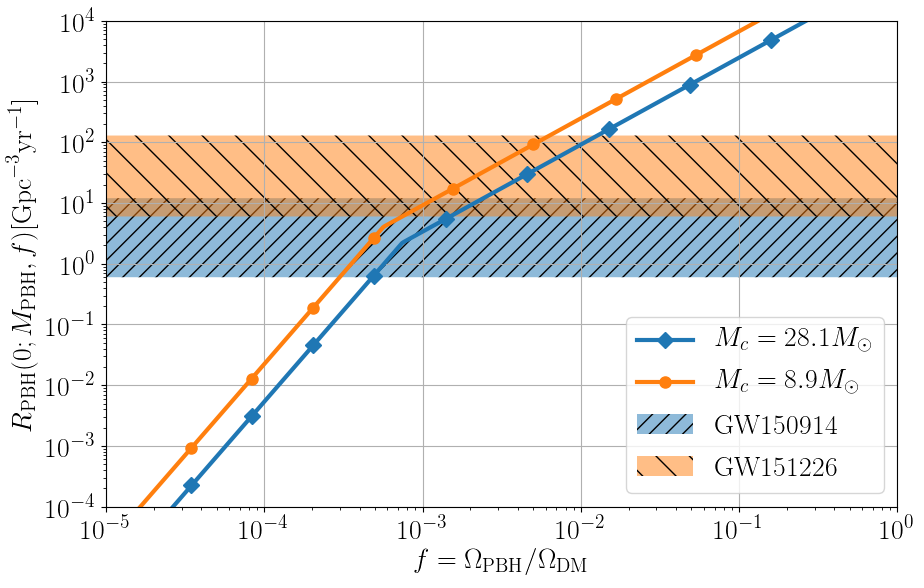
\includegraphics[width=\columnwidth]{PBH-localrate.png}
	\caption{The local merger rate $R_\text{PBH}(z=0;M_\text{PBH},f)$ of primordial \acp{BH} with chirp mass ${M}_c = 28.1 M_\odot$ (GW150914 like) and ${M}_c = 8.9 M_\odot$ (GW151226 like).
	As a comparison, the shaded region is the local merger rate associated with the GW150915- and GW151226-like \acp{BBH} \cite{GW150914rate,O1}.}
	\label{fig:PBH-localrate}
\end{figure}

For the primordial \ac{BH} mass spectrum, a narrow spread distribution \cite{Kawasaki:2012wr,Jedamzik:1999am,Kodama:1982sf,Khlopov:2000js} and an extended distribution \cite{Carr:1975qj,Hawking:1987bn} are both considered by early Universe models.
However, it has been shown that the inflationary scenario does not favor those with a significantly extended primordial \ac{BH} mass distribution \cite{Carr:2016drx}.
We also find that for a Gaussian primordial \ac{BH} mass distribution with a narrow width $\Delta M\sim1\mathrm{M}_\odot$ the resulting \ac{SGWB} amplitude is negligibly different (less than 1\% between $10\rm{Hz}-100\rm{Hz}$) from that by assuming a fixed mass distribution.
A later work by Ref.~\cite{Raidal:2017mfl} which generalized our constraining results also confirmed that assuming a log-normal mass distribution with variance $\sigma\sim\mathcal{O}(1)$ would not change the order of magnitude of the upper limits on primordial \ac{BH} abundance. 
Therefore, given the large uncertainties in the primordial \ac{BH} mass distribution \cite{Carr:2016drx} and aiming to investigate to which extent \ac{SGWB} can constrain the primordial \ac{BH} abundance, we follow Sasaki et al. and use the simplifying assumption that all primordial \acp{BH} have the same mass.

In contrast to binary primordial \acp{BH}, the astrophysical \ac{BBH} merger rate $R_\textrm{astro}(z)$, which is described in \textit{e.g.} Ref.~\cite{TheLIGOScientific:2016wyq}, peaks at $z=1\sim2$, because of the peak in the astrophysical star formation rate \cite{Vangioni:2014axa}.
While for the primordial \ac{BH} binaries whose mass and local merger rate are consistent with those of GW150914 and GW151226, the merger rate $R_\textrm{PBH}(z)$ keeps rising out to a large redshift (at least $z\sim30$, see \cite{Nakamura:2016hna}), due to the fact that primordial \acp{BH} form in the early Universe, and thus have a larger merger rate at high redshift than astrophysical \acp{BBH}.
A comparison of the merger rate for primordial and astrophysical \acp{BBH} is given by \cref{fig:PBH-rate}.

The merger rate as a function of redshift, especially at high redshift, can give us important information about the origin of \acp{BBH}, since $R_\textrm{PBH}(z)$ and $R_\textrm{astro}(z)$ behave differently.
Recently it has been proposed that Pre-DECIGO (Pre-DECihertz laser Interferometer Gravitational-wave Observatory) can determine the origin of GW150914-like \acp{BBH} by measuring the mass spectrum and the $z$-dependence of the merger rate \cite{Nakamura:2016hna}.
Therefore, future space-based \ac{GW} detectors, such as LISA \cite{Heinzel:2014ets,Bartolo:2016ami}, DECIGO \cite{Kawamura:2006up} and BBO \cite{Harry:2006fi}, may also be used to study the origin of \acp{BBH}.
The correlation of \ac{GW} events with galaxy catalogs may also distinguish the origin of \acp{BBH} \cite{Raccanelli:2016cud}.

\begin{figure}[htbp]
	\centering
	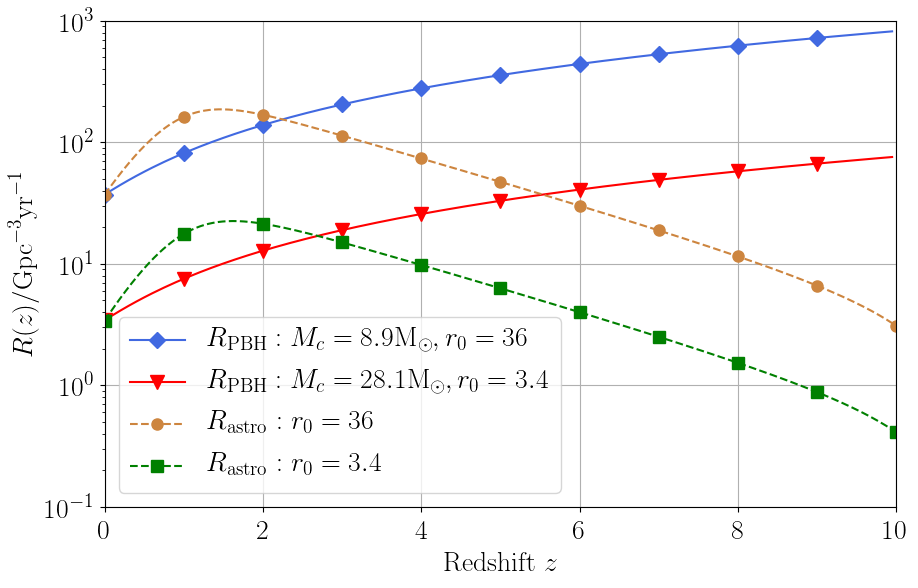
\includegraphics[width=\columnwidth]{PBH-rate.png}
	\caption{The \ac{BBH} merger rate $R(z)$ of astrophysical and primordial origin as a function of redshift $z$. 
	The local merger rate is denoted by $r_0$. 
	For the astrophysical \ac{BBH} merger rate, the ``$R_\text{astro}:r_0 = 3.4$'' corresponds to GW150914-type \ac{BBH} and considers only the metallicity $Z<Z_\odot/2$ portion of star formation rate, while the ``$R_\text{astro}:r_0= 36$'' corresponds to GW151226-type \ac{BBH} and all the metallicity is taken into account.
	For the parametrization of the star formation rate associated with different metallicity, readers can refer to, e.g., Ref.~\cite{Callister:2016ewt}.}
	\label{fig:PBH-rate}
\end{figure}

\section{Stochastic gravitational-wave background energy density spectrum} 
\noindent Given the merger rate of \acp{BBH}, one can obtain the \ac{SGWB} energy density spectrum from
\begin{equation}
\Omega_{\textrm{GW}}=\frac{\nu}{\rho_\textrm{c}}\frac{d\rho_{\textrm{GW}}}{d\nu},
\end{equation}
where $d\rho_{\textrm{GW}}$ is the gravitational radiation energy density in the frequency interval $(\nu,\nu+d\nu)$, and $\rho_c = 3H_0^2 c^2/8\pi G$ is the critical energy density of the Universe \cite{Allen:1997ad}.
For the \ac{SGWB} produced by binary primordial \ac{BH} mergers, $\Omega_{\textrm{GW}}$ can be expressed as an integral over the redshift, namely
\begin{align}
\Omega_{\textrm{GW}}(\nu;M_\textrm{PBH},f) = &\frac{\nu}{\rho_\textrm{c}H_0} \int_{0}^{z_{\textrm{sup}}} \frac{R_\textrm{PBH}(z;M_\textrm{PBH},f)}{(1+z)E(z)} \times  \\ \nonumber
& \frac{dE_\textrm{GW}}{d\nu_\textrm{s}}(\nu_\textrm{s}) \, dz,
\label{GW spectrum}
\end{align}
where ${dE_\textrm{GW}}/{d\nu_\textrm{s}}(\nu_\textrm{s})$ is the \ac{GW} energy spectrum of \acp{BBH} coalescence, $\nu_\textrm{s}$ is the frequency in source frame and is related to the observing frequency $\nu$ through $\nu_\textrm{s}=(1+z)\nu$. The factor $(1+z)$ on the denominator converts the merger rate from source frame to observer frame.
For this work, we assume an inspiral-merger-ringdown energy spectrum with non-precessing spin correction \cite{IMRPhenomA,IMRPhenomB}.
The upper limit of the integration is given by $z_{\textrm{sup}}=\min(z_{\textrm{max}},\nu_{\textrm{cut}}/\nu-1)$, where $\nu_\textrm{cut}$ is the cut-off frequency given the energy spectrum of \ac{BBH} and $z_{\textrm{max}}$ is the maximum redshift predicted by the primordial \ac{BH} model.
Since primordial \acp{BH} are formed in the early Universe, $z_{\rm max}$ is larger than $\nu_{\textrm{cut}}/\nu-1$ so that $z_{\rm sup}$ never takes the value of $z_{\rm max}$ in the Advanced LIGO sensitive frequency band.

Ref.~\cite{Mandic:2016lcn} investigates the \ac{SGWB} energy density spectrum from primordial \ac{BH} binaries, compares it to that from astrophysical \acp{BBH} and discusses the detectability for future \ac{GW} detectors.
The primordial \ac{BH} background was shown to have the same power law spectrum $f^{2/3}$ as that from astrophysical \acp{BBH} in the Advanced LIGO sensitivity band.
Moreover, it has been suggested that the SGWB can be used to investigate the primordial \ac{BH} abundance. 
Here, we consider the constraints on the primordial \ac{BH} abundance using the \ac{SGWB} in a different primordial \ac{BH} binary formation framework by Sasaki et al. which produces binaries in the early Universe, as opposed to that used by Ref.~\cite{Mandic:2016lcn} which forms binaries in the late Universe.
Since the primordial \acp{BH} in the early Universe are distributed more densely, the Sasaki et al. framework has a larger merger rate, leading to a stronger \ac{SGWB} amplitude compared with Ref.~\cite{Mandic:2016lcn}.

\begin{figure}[htbp]
	\centering
	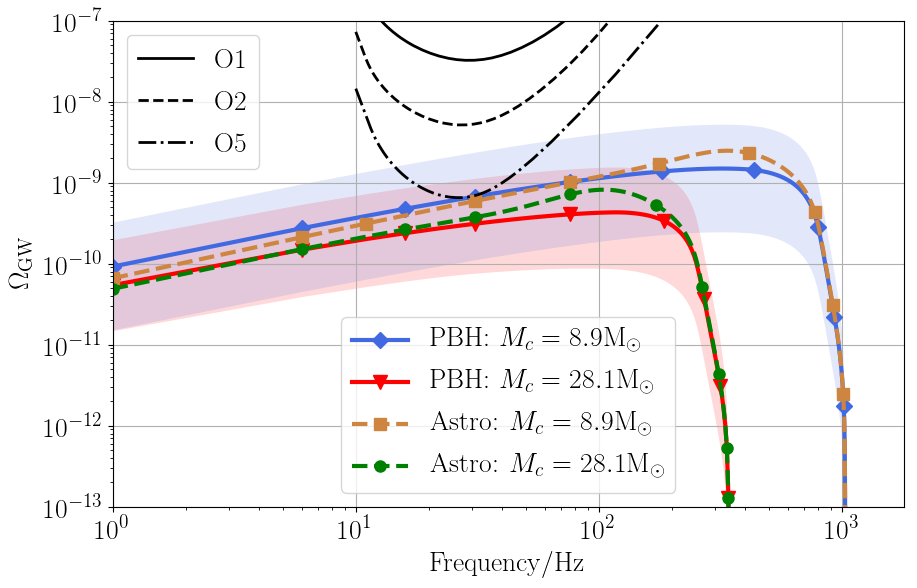
\includegraphics[width=\columnwidth]{PBH-SGWB.png}
	\caption{The \ac{SGWB} energy density spectra as a function of the observed frequency and the expected sensitivities of Advanced LIGO’s O1, O2 and O5. 
	The chirp mass and local merger rate of the primordial \acp{BH} are assumed to be the same as the estimation of the GW150914 and GW151226 events. 
	The different cut-off frequency of SGWB from $M_c = 8.9M_\odot$ is due to the different choice of symmetric mass ratio and effective spin parameter.}
	\label{fig:PBH-SGWB}
\end{figure}

\cref{fig:PBH-SGWB} shows the \ac{SGWB} energy density spectra due to binary primordial \ac{BH} mergers as a function of observed frequency.
For the primordial \ac{BH} binaries, we employ the identical chirp mass and local merger rate to the \ac{GW} events, but assume non-spinning and equal component mass binaries. 
For comparison, we also illustrate the \ac{SGWB} spectra of astrophysical \ac{BBH} origin here. 
The shaded regions denote the $90\%$ statistical uncertainties, due to the propagation of uncertainty from the local merger rate. 
The black curves denote the $1\sigma$ sensitivity of the LIGO-Virgo network expected for two first observing runs O1 (black solid) and O2 (black dashed), and at the design sensitivity in O5 (black dot-dashed) \cite{TheLIGOScientific:2016wyq,Thrane:2013oya}. 
The sensitivity curve is calculated in the context of the cross correlation statistic method \cite{Allen:1997ad} with one year of integration, and the coincident duty cycle is $30\%$ for O1 and $50\%$ for O2 and O5. 
If a model-predicting spectrum intersects a black curve, then it has an expected \ac{SNR} greater or equal than 1.

From \cref{fig:PBH-SGWB}, the \ac{SGWB} energy density spectrum from binary primordial \ac{BH} mergers looks very similar to that of astrophysical origin. 
We also notice a bump feature around the peak of the \ac{SGWB} spectrum from astrophysical \ac{BBH}
mergers due to the peak of star formation rate. 
This feature might help us to distinguish primordial \acp{BH} from astrophysical \acp{BH}.
However, the Advanced LIGO detector does not have the sensitivity required to observe the bump \cite{Callister:2016ewt}.

\section{Constraining the primordial black hole abundance with the stochastic gravitational-wave background} 
Since the first Advanced LIGO observation run did not find evidence for a \ac{SGWB} signal \cite{TheLIGOScientific:2016dpb}, we can use the non-detection to constrain the maximum \ac{SGWB} energy density spectrum $\Omega_{\textrm{GW}}^{\textrm{max}}(\nu)$, and to further constrain the maximum primordial \ac{BH} abundance $f_\textrm{max}$ by equating
\begin{equation}
\Omega_{\textrm{GW}}^{\textrm{max}}(\nu) = \Omega_{\textrm{GW}}(\nu;M_\textrm{PBH},f_\textrm{max}),
\end{equation}
thereby giving a upper limit $f_\textrm{max}$ on the primordial \ac{BH} abundance for different $M_\textrm{PBH}$. 
Taking advantage of the unique observational window from \ac{GW}, the \ac{SGWB} yields a new independent constraint on the properties of primordial \acp{BH} which we can compare to other methods, such as lensing of stars and quasars, dynamics of dwarf galaxies, large scale structure and accretion effects on the \ac{CMB} \cite{Carr:2016drx}. 

\begin{figure}[htbp]
	\centering
	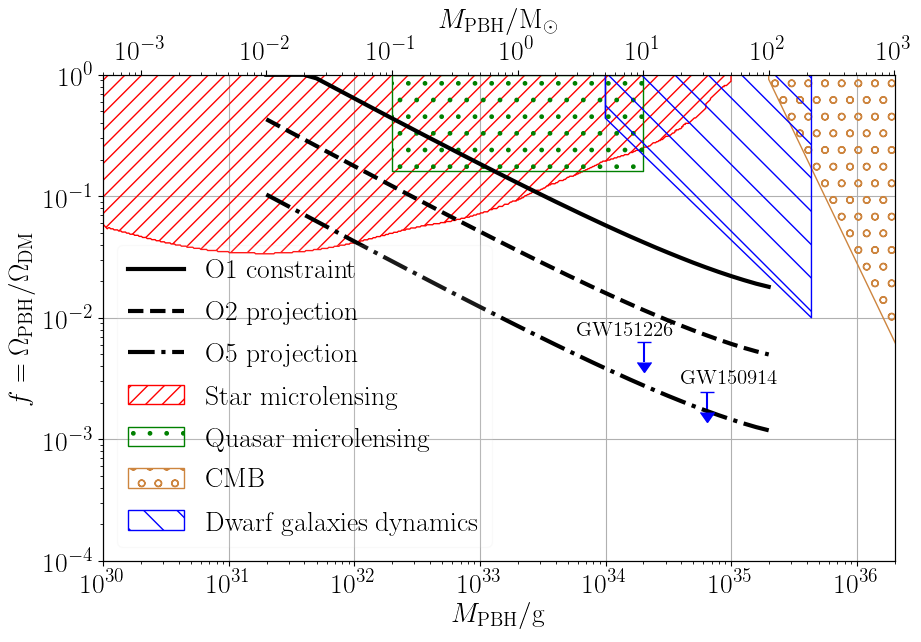
\includegraphics[width=\columnwidth]{PBH-constraint.png}
	\caption{
		The constraints on the primordial \ac{BH} fraction in dark matter $f_\textrm{max}$ versus the primordial \ac{BH} mass $M_{\rm PBH}$ from the non-detection of the \ac{SGWB} from Advanced LIGO's O1 observation run and the expected constraints based on the O2 and O5 projected sensitivities.
		These constraints are compared to those from star microlensing \cite{Novati:2013fxa}, quasar microlensing \cite{Mediavilla:2009um}, dynamics of dwarf galaxies \cite{Koushiappas:2017chw} and accretion effect on \ac{CMB} \cite{Ali-Haimoud:2016mbv}.
		The local merger rate for GW150914 and GW151226-like \ac{BBH} can also constrain the primordial \ac{BH} abundance with corresponding mass. 
	}
	\label{fig:constraint}
\end{figure}

\Cref{fig:constraint} shows the current upper limit in the $f$-$M_{\textrm {PBH}}$ plane from Advanced LIGO's O1 (2015-16, black solid), and the expected constraints from O2 (2016-17, black dashed) and O5 (2020-22, dot-dashed).

For comparison, constraints on $f$ from the EROS/OGLE microlensing of stars\footnote{This result is obtained by combining EROS and OGLE detections and achieved tighter constraints by  assuming that a few positive detections from OGLE are explained by self-lensing.} \cite{Novati:2013fxa} , microlensing of quasars \cite{Mediavilla:2009um}, dynamics of dwarf galaxies \cite{Koushiappas:2017chw} and accretion effect on \ac{CMB} \cite{Ali-Haimoud:2016mbv} are also plotted. 

In addition, the inferred local merger rates associated with the GW150914 and GW151226 like \acp{BBH} can also constrain the abundance of primordial \ac{BH}. Since we adopt a delta primordial \ac{BH} mass distribution following Sasaki et al. given the large theoretical uncertainty, for consistency, we also consider the LIGO's local merger rate estimated by assuming all the black holes have the same mass as detected rather than an extended distribution. By imposing the condition that $R_{\textrm{PBH}}(z=0;M_\text{PBH},f_\textrm{max})$ can not exceed the maximum of the estimated local merger rate, a upper limit on the primordial \ac{BH} abundance $f_\textrm{max}$ can be given with corresponding $M_\textrm{PBH}$, as shown in \Cref{fig:constraint}.

We see that up to now microlensing gives the tightest constraints in mass range $10^{-3}\mathrm{M}_\odot\lesssim M_\text{PBH}\lesssim 1 \mathrm{M}_\odot$. The new upper limit given by \ac{SGWB} from Advanced LIGO's O1 gives the best constraint on the primordial \ac{BH} abundance in the mass range $1 \mathrm{M}_\odot \lesssim M_\text{PBH}\lesssim 100 \mathrm{M}_\odot$\footnote{
primordial \ac{BH} binaries with masses higher than $\sim\mathcal{O}(10^2)M_\odot$ would have a lower cut-off frequency, thus would evade the frequency band of Advanced LIGO.},
pushing the previous microlensing and dwarf galaxies dynamics constraint tighter by one order of magnitude.
Future observing runs of Advanced LIGO are expected to improve the constraint $f_\textrm{max}$ further to $\mathcal{O}(10^{-3})$. 

Conversely, we can compare the \ac{SGWB} spectra from the current constraints to the expected Advanced LIGO sensitivities. 
\Cref{fig:ogwfm} shows the \ac{SGWB} spectra from binary primordial \ac{BH} mergers for different chirp masses using current most stringent constraints of the primordial \ac{BH} abundance.
Here the chirp mass is defined by $M_c=(m_1m_2)^{3/5}/(m_1+m_2)^{1/5}$, where $m_1$ and $m_2$ are the component mass of \acp{BBH}. Thus, $M_c = M_\textrm{PBH}/2^{1/5}$ for primordial \acp{BH} of a fixed mass.

\begin{figure}[htbp]
	\centering
	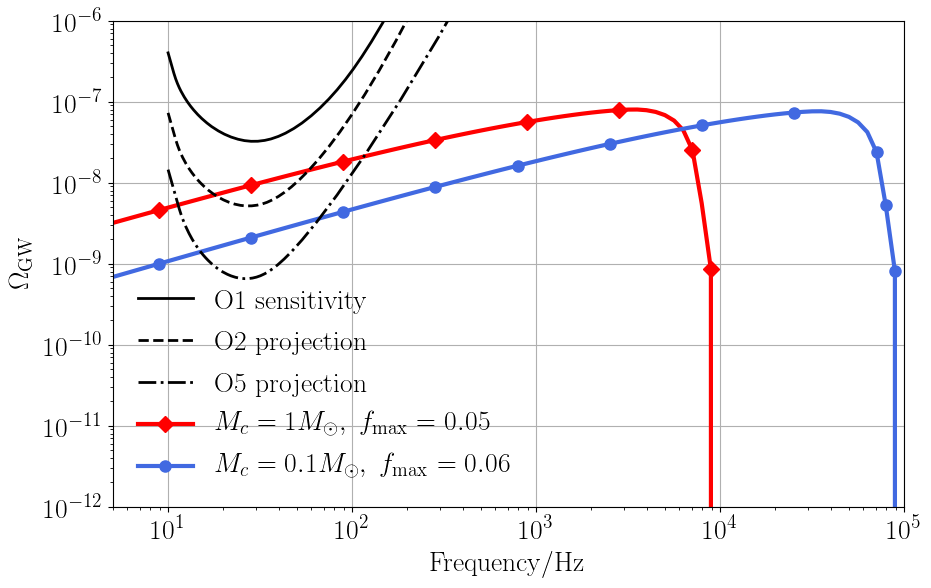
\includegraphics[width=\columnwidth]{PBH-SGWB2.png}
	\caption{
		The \ac{SGWB} spectra from sub-solar mass binary primordial \ac{BH} mergers at the current best constraints from stellar microlensing.
		Non-detection in Advanced LIGO's O2 observation can further constrain the existence of sub-solar mass primordial \acp{BH}.
	}
	\label{fig:ogwfm}
\end{figure}

From the \Cref{fig:ogwfm} we can see that the \ac{SGWB} generated by subsolar mass primordial \acp{BH} has the opportunity to be detected by upcoming Advanced LIGO observing runs.
Therefore, the SGWB provides a possible way to explore the existence of subsolar mass primordial \acp{BH}, which would be a smoking gun for the existence of primordial \acp{BH} since subsolar mass \acp{BH} are not expected to be of a stellar origin. 
However, a decisive evidence for primordial \ac{BH} would need the detection of \ac{SGWB} at high frequency which is beyond the scope of Advanced LIGO.
Nevertheless, \ac{SGWB} provides a complementary channel to investigate the properties of subsolar mass \acp{BH}, even if their \ac{GW} signal is too weak to be individually resolved.

\section{Discussion} 
\noindent In this work, we place a novel constraint on the primordial \ac{BH} abundance in dark matter in the mass range $0.01\mathrm{M}_\odot -100\mathrm{M}_\odot$ using the current non-detection of \ac{SGWB} from Advanced LIGO's first observation run.
As a new observational window, the constraint from \ac{SGWB} is better than other methods such as microlensing and dwarf galaxies dynamics by one order of magnitude in the mass range $1 \mathrm{M}_\odot \lesssim M_\text{PBH}\lesssim 100 \mathrm{M}_\odot$.
Finally, we also find that the current most stringent constraints on the abundance of subsolar mass primordial \acp{BH} can give a measurable \ac{SGWB} by future Advanced LIGO observing runs.

The coalescence of a binary primordial \acp{BH} produces a BH of higher mass, and this evolution of the mass distribution has an effect on the \ac{SGWB} spectrum.
Nevertheless, at the matter-radiation equality epoch $z_\mathrm{eq}$, only a pair of primordial \acp{BH} which satisfies $x<f^{1/3} \bar x$ can form a binary \cite{Sasaki:2016jop}, where $x$ is the physical separation between two neighboring primordial \acp{BH}.
This means that the fraction of primordial \acp{BH} which can form binaries in the total primordial \ac{BH} population is $x^3_{\mathrm{max}}/{\bar x}^3 \simeq f$.
Thus, the fraction of subsequent more-massive primordial \ac{BH} binaries in the original population of primordial \ac{BH} binaries is also given by $f$.
From \cref{fig:constraint}, the typical value of $f_\textrm{max}$ is of the order of $\mathcal{O} (0.01)$.
However, the mass doubling effect will only contribute an extra factor of $2^{5/3}\sim3$ 
to the \ac{GW} energy density spectrum ($dE/d\nu\propto M_\textrm{c}^{5/3}$).
Therefore, we expect that the evolution of the mass distribution has a negligible effect on the \ac{SGWB} in this work's scenario.
However, we also notice that primordial \acp{BH} may be clustered in the late Universe, boosting the formation rate of more-massive primordial \ac{BH} binaries.
The effect of such clustering is beyond the scope of this paper and is left for a future work.

Another consideration is that primordial \ac{BH} binaries may be formed with highly eccentric orbits, and these binaries could preserve the eccentricity until merger if they coalesce on time scales within years or less \cite{Cholis:2016kqi,Clesse:2016ajp}.
In this work, the contribution of primordial \ac{BH} mergers to the \ac{SGWB} spectrum in the Advanced LIGO sensitive frequency band comes from the redshift $z<\nu_{\textrm{cut}}/\nu-1$.
Compared with the binary formation epoch which is earlier than the matter-radiation epoch $z_\mathrm{eq}$, the primordial \ac{BH} binaries are expected to have enough time to circularize the orbits.
Therefore, we assume that the effects of eccentricity are negligible when calculating the \ac{SGWB} in this work.
However, when considering a lower frequency band, one should include the influence of the gravitational-wave emission from eccentric binaries (see, \textit{e.g.} Ref.~\cite{Yunes:2009yz,PhysRevD.90.084016,Mikoczi:2015ewa,Tanay:2016zog,Mishra:2015bqa,PhysRevD.95.024038,Chen:2016zyo}) on the \ac{SGWB}.

%\textit{version 2: }{\color{red}
%It should also be noted that the primordial \ac{BH} abundance constraints put by this work rely on the merger rate of Sasaki et al., which in turn assumes that binaries formed at early times and not merged yet survive until $z=0$.
%We notice that the study on this question is in continuous progress, \textit{e.g.}, a recent work Ref.~\cite{Ali-Haimoud:2017rtz} showed supportive arguments that primordial \ac{BH} binaries are mostly unaffected by their environment between formation and merger.
%Nevertheless, more investigations are needed to fully understand the evolution of binary primordial \ac{BH} in the late Universe.
%As a new observational window, future \ac{GW} measurements will shed light on this question.}

Finally, our results depend on the merger rate of Sasaki et al., which in turn assumes that binaries formed at early times and not merged yet survive until $z=0$. 
The primordial \ac{BH} binary formation and evolution are still under active investigation (see, \textit{e.g.} Ref.~\cite{Hayasaki:2009ug,Eroshenko:2016hmn,Ali-Haimoud:2017rtz}).
Future \ac{GW} measurements will further shed light on the primordial \ac{BH} scenario.

Recently, three more \ac{GW} events from \ac{BBH} merger, GW170104, GW170608 and GW170814, were announced during the second Advanced LIGO-Virgo observation run \cite{PhysRevLett.118.221101,Abbott:2017gyy,PhysRevLett.119.141101} \footnote{After the accomplishment of this work, more \ac{GW} events are found in the first and second observation runs, as reviewed in \cref{ch:review1}.}.
In the absence of a publicly available event rate statement from each event alone and \ac{SGWB} results for the second observation run, we leave this analysis for future work.

\chapterend

\chapter{Constraining Primordial Black Hole Abundance with the Stochastic Gravitational-Wave Background in the Space-Based Detector Frequency Band}\label{chap:SGWBspace}

\section{Introduction} 

\subsection{An Overview of the Main Idea}
In this chapter, we focus on the \ac{SGWB} from primordial \acp{BH} in the space-based detector frequency band ($[10^{-5}, 10^{-1}]$ Hz).
The main idea is as follows.
Assuming that primordial \acp{BH} compose a fraction of dark matter, some of them may accumulate  at the center of galaxy and perform a prograde or retrograde orbit against the gravity pointing towards the center exerted by the central massive \ac{BH}.
If the mass of primordial \acp{BH} is of the order of stellar mass or smaller, such \acp{EMRI} can emit \acp{GW} and form a background due to incoherent superposition of all the contributions of the Universe. 
We investigate the \ac{SGWB} energy density spectra from the directional source, i.e., the primordial \acp{BH} surrounding Sagittarius A$^\ast$ of the Milky Way, and the isotropic extragalactic total contribution, respectively.
As will be shown in the following section, the resultant \ac{SGWB} energy density show different spectrum features such as the peak positions in the frequency domain for the above two kinds of sources.
Detection of \ac{SGWB} with such a feature may provide evidence for the existence of primordial \acp{BH}. 
Conversely, a null searching result can put constraints on the abundance of primordial \acp{BH} in dark matter.

\subsection{Primordial Black Holes as Dark Matter at the Galactic Center}

The recent direct detections of \ac{GW} by LIGO and Virgo collaboration opens a unique window to observe \acp{BH}
\cite{Abbott:2016blz,Abbott:2016nmj,O1,Abbott:2017vtc,Abbott:2017oio,TheLIGOScientific:2017qsa,Abbott:2017gyy,GWTC1}.
The event rate of binary \ac{BH} merger at local Universe is estimated to be $53.2^{+58.5}_{-28.8}$ Gpc$^{-3}$ yr$^{-1}$ from the detections \cite{GWTC1-rate}. 
Among the \ac{GW} events, the relatively large mass of the first detection ($\sim 30 M_\odot$), GW150914, has stimulated discussions that the binary \acp{BH} of GW150914 could be of primordial origin, instead of products of stellar evolution \cite{Bird:2016dcv,Clesse:2016vqa,Sasaki:2016jop}.
Ref.~\cite{Sasaki:2016jop} shows that the binary stellar-mass primordial \acp{BH} coalescence scenario can give the correct order of magnitude of event rate, if the abundance of primordial \acp{BH} in dark matter is $\sim10^{-3}$.

Primordial \acp{BH} are a long hypothesized candidate for dark matter \cite{Hawking:1971ei,Carr:1974nx,PBH1993-Silk,PBH1996}. 
Assuming all the primordial \acp{BH} have the same mass, a variety of observations from astronomy and cosmology have given constraints on the primordial \ac{BH} abundance in dark matter, for example, gravitational lensing of stars and quasars, dynamics of dwarf galaxies, large scale structure formation and accretion effects on the \ac{CMB} (see Refs.~\cite{Carr:2016drx,Sasaki:2018dmp} and references therein). 
The possibility that all the dark matter are primordial \acp{BH} with the same mass has been ruled out given all the constraints aforementioned.
Nevertheless, it is still interesting to consider the scenario where primordial \acp{BH} compose a part of dark matter and propose new methods to seek for evidence of primordial \acp{BH} or constrain their abundance in dark matter.

In this work, we investigate the scenario in which primordial \acp{BH} constitute a fraction of dark matter in the galactic center.
Astrophysical observations (see, e.g., Refs.~\cite{SMBH-Review-2,SMBH-Review-1} for a review) indicate that massive \acp{BH} with mass $10^5 M_\odot- 10^{9} M_\odot$ are ubiquitous and reside at the center of almost every massive galaxy. 
If some fraction of dark matter is composited by  primordial \acp{BH}, they should perform a prograde or retrograde orbit against the gravity pointing towards the galactic center exerted by the central massive \ac{BH}, and such a system becomes the so-called \ac{EMRI} system whose mass ratio is usually larger than $10^5$ \cite{Babak:2017tow}.
\acp{EMRI} are one of the important scientific targets of space-based \ac{GW} detector, such as \ac{LISA} which is anticipated to be launched in the 2030s \footnote{https://www.elisascience.org/}.
Once detected, the \ac{GW} signals from \acp{EMRI} can provide valuable information such as event rate estimation \cite{Babak:2017tow,AmaroSeoane:2010bq} and tests of general relativity \cite{Barack:2006pq,Gair:2012nm}.

The focus of our work is the \ac{SGWB} energy density spectrum from \ac{EMRI} system consisting of a massive \ac{BH} at the galactic center and a sub-solar mass primordial \ac{BH}.   
\ac{SGWB} is an incoherent superposition of numerous \acp{GW}, including those too weak to be detected individually \cite{Regimbau:2011rp,SGWBlivingreview,TheLIGOScientific:2016wyq,TheLIGOScientific:2016dpb,Abbott:2017xzg} or having intrinsic stochastic nature such as primordial \ac{GW} is generated by quantum fluctuations in the early Universe. 
The \ac{SGWB} from binary stellar-mass primordial \ac{BH} coalescence is calculated by Refs.~\cite{Mandic:2016lcn,Wang:2016ana,Chen:2018rzo,Clesse:2016ajp} and, in particular, Ref.~\cite{Wang:2016ana} shows that the null result of \ac{SGWB} in the LIGO frequency band ($[10,1000]$ Hz) has given the most stringent constraints on the abundance of primordial \ac{BH} as dark matter in the mass range $[1,100] ~M_\odot$.
In the \ac{LISA} frequency band, 
Ref.~\cite{Guo:2017njn} have investigated the individually resolvable \ac{GW} signals from the primordial \ac{BH}-massive \ac{BH} interacting systems up to redshift $z =1$. 
Refs.~\cite{Kuhnel:2017bvu, SgrA} have considered the stochastic background from sub-solar mass primordial \acp{BH} inspiraling to Sagittarius A$^\ast$, i.e., the central massive \ac{BH} of the Milky Way. 
Our work will expand the study of Refs.~\cite{Kuhnel:2017bvu, SgrA} in the following two aspects. First, we  calculate the \ac{SGWB} energy density spectrum in the frequency domain, i.e., $\Omega_\text{GW}(\nu)$ from the primordial \acp{BH} surrounding Sagittarius A$^\ast$. Second, we investigate the complete \ac{SGWB} contributions from extragalactic sources by modeling the event rate of primordial \ac{BH} \acp{EMRI} throughout the cosmic redshift.
% and presenting the results of \ac{SGWB} spectra.

In \cref{sec:sgrA} we model the primordial \acp{BH} density profile around a massive \ac{BH}, and apply this relation to the Sagittarius A$^\ast$ in the Milky Way to derive the \ac{SGWB} energy density spectrum.
We proceed to model the number density of massive \acp{BH} at different redshift epoch and calculate the \ac{SGWB} spectrum from extragalactic sources in \cref{sec:extragalactic}.
We forecast the ability of \ac{LISA} for detecting the \ac{SGWB} signal or, if there is a null result, constraining the abundance of primordial \acp{BH} in dark matter in \cref{sec:PBH-EMRI-constraint}.
The results show that \ac{LISA} can probe the existence of primordial \acp{BH} with mass range $[10^{-8} , 1 ]~M_\odot$ and constrain the abundance of primordial \ac{BH} with $1 M_\odot$ to be $10^{-9}$ in the optimal case where the dark-matter spike scenario with a steeper initial power index $\gamma=2$ is valid.
The main uncertainty is subject to the value of the dark-matter initial power index $\gamma$.
We summarize the conclusions in \cref{sec:PBH-EMRI-conclusion}.
Throughout this work we assume the mass distribution of primordial \acp{BH} is a delta function due to the uncertainty of primordial \ac{BH} population.
Therefore the results should be seen as being from the primordial \acp{BH} with a representative mass.
Actually, as will be shown in the following, the mass of primordial \acp{BH} only serves as a scaling factor for the amplitude of the resulting \ac{SGWB} spectra and the shape of spectra only depends on the mass of the central massive \acp{BH}.

\section{The Stochastic Gravitational-Wave Background from Sagittarius A$^\ast$}\label{sec:sgrA}
\subsection{Primordial Black Holes Density Profile} 
To model the event rate of primordial \ac{BH} \acp{EMRI}, we first infer the primordial \ac{BH} mass density at the galactic center. 
Since we expect that primordial \acp{BH} compose a part of dark matter, it is natural to use the dark-matter density profile to characterize the primordial \ac{BH} mass density around the central massive \ac{BH}.

For an initial dark-matter density profile with the following power law form
\be\label{Eq:powerindex}
\rho(r) = \rho_0\left(\frac{r_0}{r}\right)^{\gamma},
\ee
where $\rho_0$ and $r_0$ are halo parameters and to be determined, $\gamma$ is the power index, $r$ is the radius of dark matter, Ref.~\cite{PhysRevLett.83.1719} suggests that the adiabatic growth of  the central massive \ac{BH} can enhance the surrounding dark-matter density at galactic center and form a spike distribution, i.e., the halo will end up with the following density \cite{PhysRevLett.83.1719,Nishikawa:2017chy}
\be \label{eq:spike}
\rho_\text{sp}(r) = \rho_R \left( 1-\frac{4R_s}{r}\right)^3\left(\frac{R_\text{sp}}{r}\right)^{\gamma_\text{sp}},
\ee 
where the power index is enhanced from the initial value by $\gamma_\text{sp} = (9-2\gamma)/(4-\gamma)$, the halo parameter $\rho_R = \rho_0(R_\text{sp}/r_0)^{-\gamma}$ with $R_s$ being the Schwarzchild radius of the central massive \ac{BH}, $R_\text{sp}(\gamma,M_\text{MBH}) = \alpha_\gamma r_0(M_\text{MBH}/(\rho_0 r_0^3))^{1/(3-\gamma)}$ is the radius to which the dark-matter spike extends, $\alpha_\gamma$ is derived numerically for different $\gamma$ in Ref.~\cite{PhysRevLett.83.1719}. 
For an initial Navarro-Frenk-White (NFW) profile \cite{NFW} with $\gamma=1$, the final spike has a index $\gamma_{\textrm{sp}}=7/3$, thus significantly boosting the inner profile around the central massive \ac{BH}.
%The dark matter spike distribution is originally proposed and calculated using Newtonian mechanics with relativistic correction by Ref.~\cite{PhysRevLett.83.1719} and revised by full general relativistic analysis by Ref.~\cite{PhysRevD.88.063522,PhysRevD.96.083014}. 

To connect $\rho_0$ and $r_0$ with the massive \ac{BH}'s property, we employ the relation among the dark-matter halo virial mass $M_\text{vir}$, the concentration parameter $c_\text{con}\equiv r_\text{vir}/r_0$ where $r_\text{vir}$ is the halo virial radius, and the mass of massive \ac{BH} $M_\text{MBH}$. 
The relation of $c_\text{con}-M_\text{vir}$ for NFW profile is given by Ref. \cite{Dutton:2014xda}
\begin{equation}\label{eq:c}
\log {c_\text{con}} = a + b \log{ \frac{M_\text{vir}}{10^{12}h^{-1}M_\odot}    },
\end{equation}
where $a = 0.520+0.385\exp(-0.617z^{1.21})$ and $b = -0.101 + 0.026z$ are numerical factors at redshift $z$.
The parametrized formula \cref{eq:c} is obtained by numerically fitting to a suite of N-body simulations for NFW profile with \textit{Planck} 2013 cosmological parameters \cite{Planck2013} in the redshift range $[0,5]$.

The mass of the central massive \acp{BH} has a correlation with a few characteristic quantities of the host galaxy, such as the velocity dispersion $\sigma$ in the spheroidal region and the total mass of the host galaxy, indicating a co-evolution history with the whole galaxy. 
By employing the observational $M_\textrm{MBH}-\sigma$ relation and using  the quasar luminosity function to link $\sigma$ with the halo mass, Ref.~\cite{Croton:2009zx} gives a parametrized relation between the massive \ac{BH}'s mass $M_\textrm{MBH}$ and the host dark-matter halo's virial mass $M_\text{vir}$,
\begin{align}
\log \left( \frac{M_\text{MBH}}{10^8 h^{-1} M_\odot}\right) &= (-2.66\pm 0.33) +(1.39 \pm  0.22) \nonumber \\
 &\times \log 	\left[  \beta^3  H(z) \left( \frac{M_\text{vir}}{10^{13} h^{-1} M_\odot }\right)\right].
 \label{Eq:MBH}
\end{align}
Here $H(z)=H_0 \sqrt{\Omega_m(1+z)^3+\Omega_\Lambda}$ is the Hubble parameter at redshift $z$ , $\Omega_m$ and $\Omega_\Lambda$ are the matter and dark energy fractional densities, respectively. $\beta$ is a ratio between the dark-matter halo's circular velocity and virial velocity, whose value is of order unity.
%The parametrized formula Eq. (\ref{Eq:MBH}) is shown to be consistent with the $z \sim 0$ $M_\textrm{MBH}-M_\text{vir}$ relation given in \cite{MBH1,MBH2}.
\cref{eq:c} together with \cref{Eq:MBH} can fix the corresponding coefficients of NFW density profile and NFW induced spike profile given the mass of massive \ac{BH}.
 
  \begin{figure}[htbp] %  figure placement: here, top, bottom, or page
   \centering
   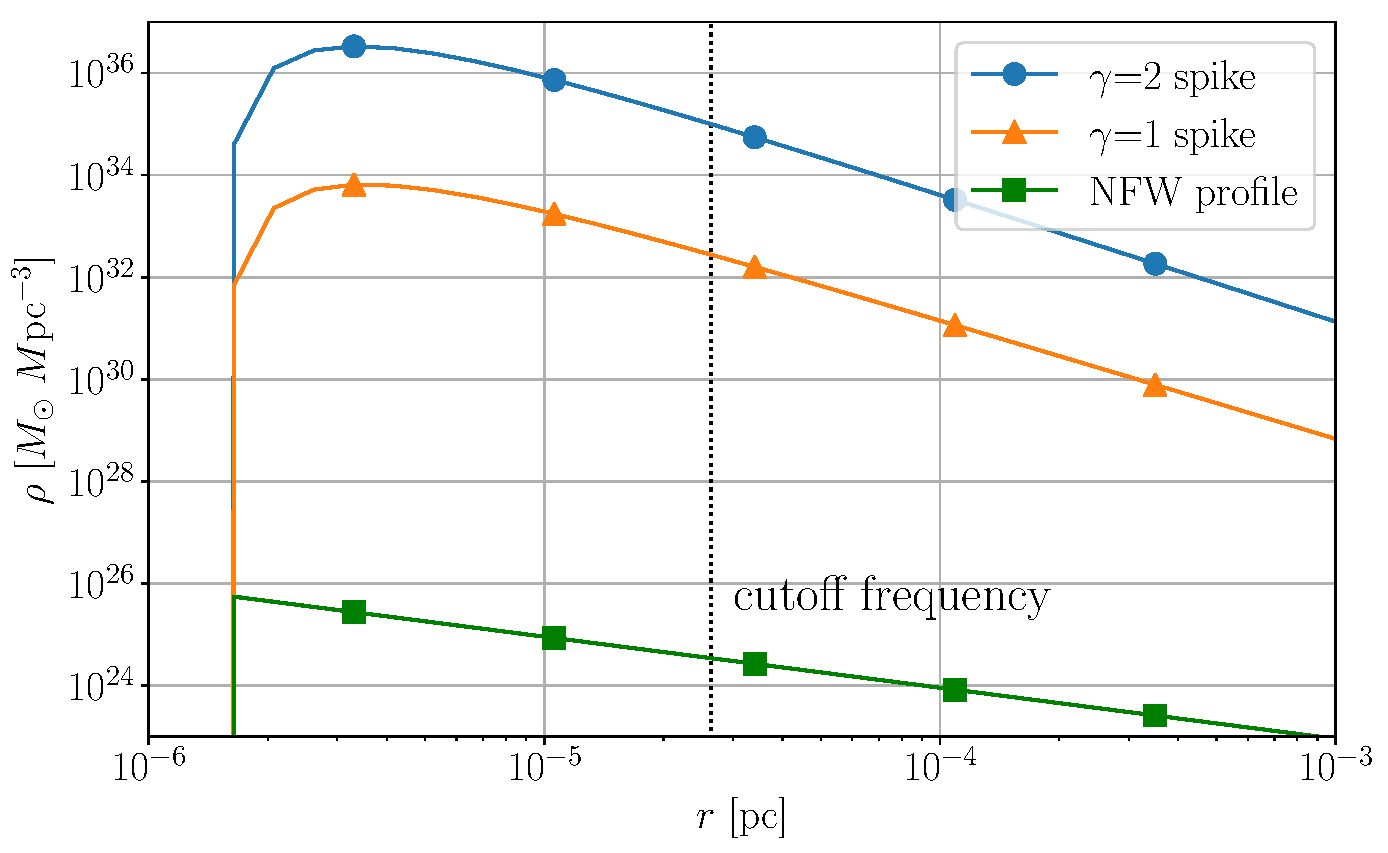
\includegraphics[width=\columnwidth]{dmprofile-sgrA.pdf} 
   \caption{Dark matter density profile around a massive \ac{BH} with mass $4\times 10^6 M_\odot$. The blue and orange solid curves show the spike profile for power index $\gamma = 2$ and $\gamma=1$, respectively. 
 As a comparison, the NFW dark-matter profile is also plotted.
The dark-matter density profile at galactic center is  boosted significantly for the $\gamma=1$ spike profile compared with the NFW profile. 
The $\gamma=2$ spike has even larger density than $\gamma=1$ by three order of magnitude.
The vertical dash line represents the orbital radius where the \ac{GW} frequency is $10^{-5} $Hz which is the lower cutoff frequency of the LISA sensitive band.
}
   \label{fig:profile}
\end{figure}

\cref{fig:profile} shows the dark-matter spike profile around a massive \ac{BH} with mass $4\times 10^6 M_\odot$.
Given the uncertainty of the initial profile power index, we choose two values for $\gamma$, $\gamma=1$ for NFW profile and $\gamma=2$ representing a steeper profile for an optimistic result.
We observe that the dark-matter density near the galactic center is  boosted significantly for the $\gamma=1$ spike profile compared with the NFW profile. 
The $\gamma=2$ spike has even larger density than $\gamma=1$ by three order of magnitude.
%The \ac{GW} dissipation induced orbital decay further enhances the dark matter density close to the central massive \ac{BH}.

In \cref{fig:profile}, the vertical dash line represents the radius where the emitted \ac{GW} frequency is $10^{-5}$ Hz under the assumption of circular motion.
Therefore the region of interest for LISA frequency band is between $4 R_s$ as indicated by \cref{eq:spike} and the dash line.

 \subsection{Stochastic Gravitational-Wave Background Spectrum}

The fractional energy density spectrum of \ac{SGWB} is defined as
\begin{equation}
\Omega_\textrm{GW} = \frac{\nu}{\rho_c}\frac{d\rho_\textrm{GW}}{d\nu},
\end{equation}
where $d\rho_\textrm{GW}$ is the gravitational-wave energy density in the frequency band $[\nu,\nu+d\nu]$, $\rho_c=3H_0^2c^2/8\pi G$ is the critical energy to close the Universe.

The local energy density is related to the \ac{GW} energy flux by $\rho_\text{GW}(\nu) = F_\text{GW}(\nu)/c$.
$F_\text{GW}(\nu)$ from Sagittarius A$^\ast$ can be derived by taking integral of the density of primordial \ac{BH} \ac{EMRI} with respect to orbital radius $r$,
\begin{equation} \label{Eq:Fgw}
F_\text{GW}(\nu) = \int{f_\text{PBH}\rho_\text{DM}(r;M_\text{MBH})\over m_\text{PBH}} {dE/dt(r;M_{tot},\eta) \over {d_L^2}}r^2 dr, 
\end{equation}
where $d_L$ is the luminosity distance from sources to \ac{GW} detectors, $\rho_\text{DM}(r;M_\text{MBH})$ is the dark-matter density  at radius $r$ to the center given $M_\text{MBH}$, $m_\text{PBH}$ and $f_\text{PBH}$ are the primordial \ac{BH} mass and abundance.
%{\color{red}As mentioned, we assume the primordial \acp{BH} perform circular Keplerian motion around the center which is determined by the mass of the central massive \ac{BH}, since the enclosed dark matter mass is negligibly small for the orbiting primordial \ac{BH}.}
% due to circularization induced by the adiabatic growth of central massive \ac{BH} \cite{Ullio:2001fb}.
To the leading order, \ac{GW} power can be calculated by the quadrupole formula \cite{peter1,peter2},
\be
\frac{dE}{dt}(r;M_{tot},\eta)=\frac{32}{5}\frac{G^4}{c^5}\eta^2\left(\frac{M_{tot}}{r}\right)^5.
\ee
%We also find that more accurate formula up to second post-Newtonian correction will give the final \ac{SGWB} result an $\mathcal{O}(1)$ correction.
%Here we use 2PN to calculate the \ac{GW} energy rate:
%\begin{eqnarray}
%-\frac{dE}{dt}(r,& M,\eta)=\frac{32}{5}\eta^2\left(\frac{Gm}{c^2r}\right)^4\frac{mc^3}{r}[1-\frac{Gm}{c^2r}\left(\frac{2927}{336}+\frac{5}{4}\eta\right)\\ \nonumber
%&+\left(\frac{Gm}{c^2r}\right)^{3/2}4\pi+\left(\frac{Gm}{c^2r}\right)^2\left(\frac{293383}{9072}+\frac{380}{9}\eta\right)]
%\end{eqnarray}
The radius $r$ can be equivalently replaced by the \ac{GW} frequency $\nu$ under the assumption of Keplerian motion,
\be\label{Eq:Kepler}
r(\nu,M_{tot})=\left[{(GM_{tot})^{1/2}\over \pi (1+z)\nu}\right]^{2\over 3}, 
\ee
where the factor of $(1+z)$ accounts for the cosmological expansion and the \ac{GW} frequency $\nu$ is twice of the orbital frequency.
From \cref{Eq:Kepler} a differential relation can  be derived ,
\be\label{Eq:differential}
{d\over d\nu}=-{2\pi\over 3}{1+z\over (GM_{tot})^{1/2}} r^{5/2}{d\over dr}.
\ee
Applying \cref{Eq:differential} to \cref{Eq:Fgw} and using the condition $M_\text{MBH}\gg m_\text{PBH}$, the differential \ac{GW} power from Sagittarius A$^\ast$ is
\be\label{Eq:dFoverdnu}
\frac{dF_\text{GW}}{d\nu}(\nu) = \frac{64\pi}{15} \frac{(1+z)G^{7/2}}{c^5}\frac{f_\text{PBH}\rho_\text{DM}m_\text{PBH}M_\text{MBH}^{5/2}}{r^{1/2}d_L^2},
\ee
Therefore the \ac{SGWB} energy density spectrum is
\begin{equation}\label{Eq:SgrA}
\Omega_\textrm{GW}^{Sgr A^{\ast}}(\nu) = \frac{\nu}{\rho_c}\frac{64\pi G^{7/2}}{15c^6} \frac{f_\textrm{PBH} m_\textrm{PBH} M_\text{MBH}^{5/2} \rho_\textrm{DM}}{ r^{1/2} d_L^2}.
\end{equation}

The mass of  Sagittarius A$^\ast$ located at the center of the Milky Way is $\sim 4\times 10^6 ~M_\odot$ and the distance $d_L$ is $\sim 8$ kpc.
Substitute the values to \cref{Eq:SgrA}, the \ac{SGWB} result is shown in \cref{fig:SgrA-Omega-GW}  with $m_\text{PBH} = 1 M_\odot$ and $f_\text{PBH} = 1\times 10^{-8}$.
Note that the term $m_\text{PBH} f_\text{PBH}$ in \cref{Eq:SgrA} only serves as an overall scaling factor.
We showcase two choices of the  initial dark-matter profile power index, $\gamma=1$ and $2$, respectively.
As a comparison, the LISA sensitivity curve of \ac{SGWB} for the six links, 5 million km arm length configuration and 5 year mission duration (the optimal case) is plotted \cite{LISAscience-phase,LISAscience-inflation}.

The figure shows that the amplitude of \ac{SGWB} with $\gamma=2$ is larger than that with $\gamma=1$ by three orders of magnitude, inheriting from the three order of magnitude difference of the dark-matter halo density as shown in \cref{fig:profile}.
Another feature is that the \ac{SGWB} peaks at $3\times 10^{-4}$ Hz, which is determined by the mass of the central massive \ac{BH} given the dark-matter spike distribution.

It should also be noted that the \ac{SGWB} from Sagittarius A$^\ast$ is a directional signal but the sensitivity curve is for isotropic \ac{SGWB}.
Therefore the comparison only serves as an order of magnitude estimation due to the lack of sensitivity curve for a directional source.
The search for persistent \ac{GW} signals from point-like sources has been performed by Advanced \cite{directional1,directional2} and Initial  \cite{directional3} LIGO and Virgo . 
Especially, using the data from the first and second observational runs of Advanced LIGO and Virgo, the upper limits for \ac{GW} strain amplitude have been given for three sources with targeting directions: Scorpius X-1, Supernova 1987 A and the Galactic Center, respectively.
Refs.~\cite{space-ansgwb1, space-ansgwb2} have considered the anisotropic \ac{SGWB} search with space-based detectors.
However, a specialized investigation for directional \ac{SGWB} from primordial \ac{BH} \acp{EMRI} at the Galactic center has not been achieved in the context of space-based \ac{GW} detectors.
We thus leave the relevant study for a future work.



  \begin{figure}[htbp] %  figure placement: here, top, bottom, or page
   \centering
   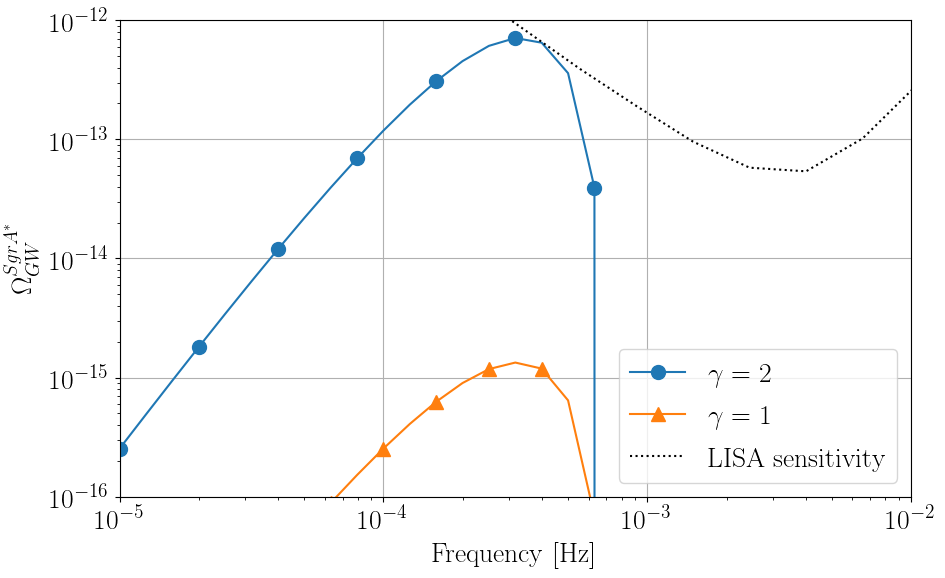
\includegraphics[width=\columnwidth]{SgrA-Omega-GW.png} 
   \caption{The \ac{SGWB} energy density spectra of primordial \ac{BH} \acp{EMRI} surrounding Sagittarius A$^\ast$, i.e., the massive \ac{BH} at the center of Milky Way. 
   The mass of primordial \ac{BH} is chosen to be $m_\mathrm{PBH} = 1 M_\odot$ and the abundance in dark matter is $f_\mathrm{PBH}$ = $10^{-8}$.
   For the initial dark-matter profile power index, $\gamma=2$ and $\gamma=1$ are chosen for illustration.
   Both \ac{SGWB} results peak at the frequency $3\times 10^{-4}$ Hz which is determined by the mass of the massive \ac{BH}.
   The amplitude with $\gamma=2$ is larger than  $\gamma=1$ by three orders of magnitude, inheriting from the three order of magnitude difference of the dark-matter halo density.
   The LISA sensitivity curve for detecting isotropic \ac{SGWB} is also plotted for a qualitative comparison since the \ac{SGWB} from Sagittarius A$^\ast$ is a directional signal.}
   \label{fig:SgrA-Omega-GW}
\end{figure}

\section{The Stochastic Gravitational-Wave Background from Extragalactic Sources} \label{sec:extragalactic}

\subsection{Massive Black Hole Population}

To model the massive \ac{BH} population throughout the cosmic history, we employ the dark-matter halo mass function and the $M_\text{MBH}-M_\text{vir}$ relation which is characterized by \cref{Eq:MBH}.
%To connect the mass of massive \acp{BH} with the dark matter virial mass,  the relation between dark matter halo virial mass and the mass of central massive \ac{BH}.
We choose the halo mass function in Ref.~\cite{Reed:2006rw} which calibrates with a suite of cosmological N-body simulations and takes the finite box size and the cosmic variance effects into account. 
In the actual practice this halo mass function  is generated through invoking the \texttt{Reed07} model in the python package \texttt{hmf} (an acronym for ``halo mass function'') \cite{Murray:2013qza}, where the cosmological parameters are set to be the value of \textit{Planck} satellite's 2018 results \cite{Planck2018}.
\texttt{Reed07} model is shown to be valid up to redshift $z\sim30$ and for halos with masses $10^{5-12} h^{-1}M_\odot$ \cite{Reed:2006rw}, which is sufficient for our purpose. 

\begin{figure}[htbp] %  figure placement: here, top, bottom, or page
   \centering
   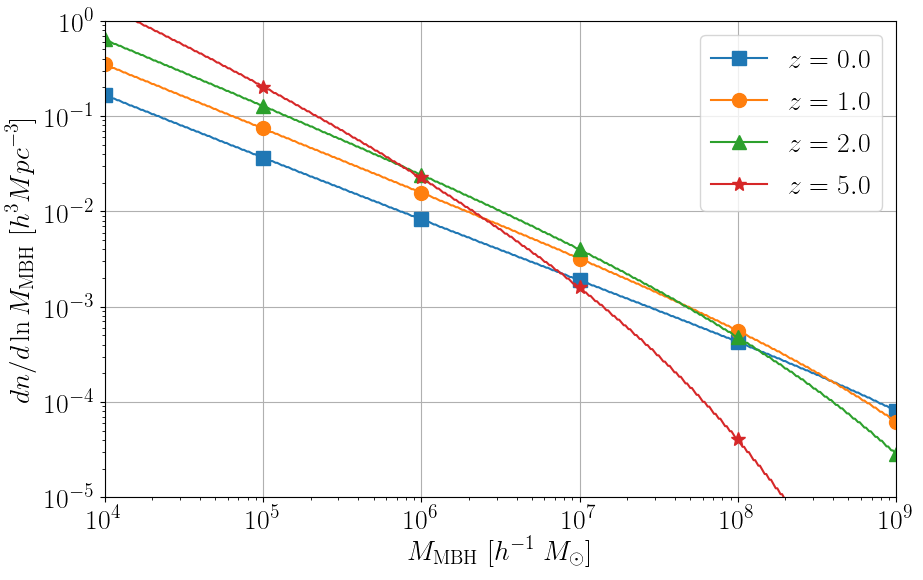
\includegraphics[width=\columnwidth]{BHmassfunction2.png} 
   \caption{The solid curves represent the number density of massive \ac{BH} at different redshifts which is derived from \texttt{Reed07} dark-matter halo mass function.
   We will consider the \ac{SGWB} spectrum from the massive \acp{BH} in the mass range $[10^4, \sim10^9]~h^{-1}M_\odot$ as a fiducial model.
   }
   \label{fig:bhmass}
\end{figure}

\cref{fig:bhmass} shows our results of the number density $dn/d\ln M_\textrm{MBH}$ for massive \acp{BH} in different redshifts. 
Since astronomical observations have confirmed the existence of massive \acp{BH} with $\sim10^{-4}~M_\odot$ (for example see Ref.~\cite{SMBH1e-4}), we will consider the \ac{SGWB} spectrum from the massive \acp{BH} in the mass range $[10^4, \sim10^9]~h^{-1}M_\odot$ as a fiducial model.
The upper mass limit is determined by the condition that the emitted \acp{GW} are in the LISA sensitive band and $\sim10^9~ M_\odot$ is sufficient for this purpose.

\subsection{Stochastic Gravitational-Wave Background Spectrum}

The complete \ac{SGWB} contribution can be obtained by taking the sum from the \acp{EMRI} of all extragalactic massive \acp{BH}
\be\label{Eq:finalOmega}
\Omega_\textrm{GW}(\nu) = \frac{\nu}{\rho_c}\frac{4\pi}{c}\iint\frac{dF_\text{GW}}{d\nu}\frac{dn}{dM_\text{MBH}}dM_\text{MBH}\chi^2 d\chi,
\ee
where $dn/dM_\text{MBH} $ is the number density of massive \acp{BH} and $\chi$ is the sources' comoving distance. Combining \cref{Eq:dFoverdnu} and \cref{Eq:finalOmega} yields
\begin{align}\label{Eq:omegacontinuous}
\Omega_\text{GW}(\nu) &= f_\text{PBH} m _\text{PBH} \frac{\nu}{\rho_c} \frac{256 \pi^2 G^{7/2} }{15 c^7}\\  \nonumber
&\times \int \frac{dz}{(1+z)H(z)} 
\int \frac{\rho_\text{DM}M_\text{MBH}^{5/2}}{r^{1/2}}   \frac{dn}{dM_\text{MBH}} dM_\text{MBH}.
\end{align}
As a fiducial model, we consider the sources in the redshift range $[0,5]$.
Contributions from higher redshift can be negligible as will be indicated in \cref{sec:robust}.

With  $m_\text{PBH} = 1 M_\odot$ and $f_\text{PBH}=10^{-8}$, the results of extragalactic \ac{SGWB}  with $\gamma=2$ and $\gamma=1$  are shown in \cref{fig:ExtGal}.
The results from Sagittarius A$^\ast$ is also replotted for comparison.
The extragalactic \ac{SGWB} peaks at a higher frequency ($\sim4\times 10^{-2}$ Hz), due to the contributions from \acp{BH} less massive than Sagittarius A$^\ast$.

\begin{figure*}[htbp]
 %  figure placement: here, top, bottom, or page
   \centering
   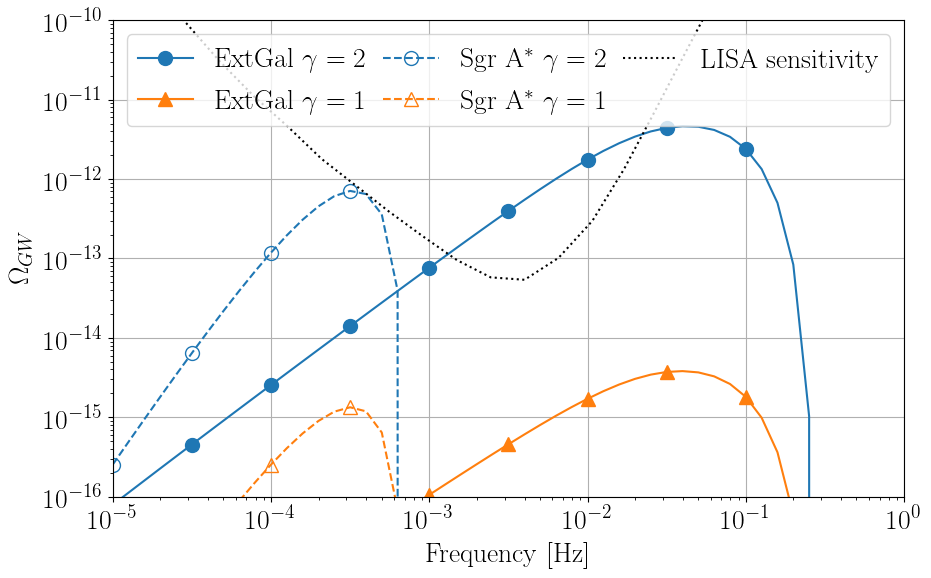
\includegraphics[width=\columnwidth]{ExtGal-Omega-GW.png}
\caption{The \ac{SGWB} spectra from primordial \ac{BH} \acp{EMRI} surrounding Sagittarius A$^\ast$ (``Sgr A$^\ast$'') and the extragalactic massive \acp{BH} (``ExtGal'') in the redshift range $[0,5]$.
The mass of the primordial \ac{BH} mass is assumed to be $1 M_\odot$ and the abundance in dark matter is $10^{-8}$. 
The dark-matter initial profile power index is chosen to be $\gamma=1$ and $\gamma=2$, respectively.
The $\gamma=2$ extragalactic \ac{SGWB} already reaches the detectable zone of LISA.
 }\label{fig:ExtGal}
\end{figure*}

Note that the extragalactic \ac{SGWB} is an isotropic signal, thus can be compared with the \ac{LISA} sensitivity curve directly. It shows that the amplitude of extragalactic \ac{SGWB}  for $\gamma=2$ already reaches the detectable zone, which means that the future LISA searching results can probe the abundance of $1 M_\odot$ primordial \acp{BH} to be as low as $\sim 10^{-9}$ for the $\gamma=2$ case.
The amplitude of $\gamma=1$ \ac{SGWB} is smaller by three order of magnitude due to a smaller dark-matter density profile.

The main uncertainty comes from the dark-matter initial profile power index. 
Future astrophysical progress on understanding the dark-matter profile at galactic center can shed light on a more robust prediction on the primordial \ac{BH} \acp{EMRI} event rate. 
Conversely, future \ac{GW} search with space-based detectors can also be beneficial for study for dark-matter profile.



\subsection{Density Enhancement due to Gravitational-Wave Dissipation}

Another consideration is that the orbit of inspiraling primordial \acp{BH} will gradually decay due to \ac{GW} dissipation. 
As a consequence, the primordial \ac{BH} density profile gets further concentrated.
To quantify this effect, we notice that astrophysical spectroscopy surveys have confirmed that the first galaxies form at redshift $z \gtrsim10$ \cite{FirstGalaxy}.
Therefore we make the most-optimistic estimation that all the primordial \acp{BH} \acp{EMRI} start to decay at $z \gtrsim 10$ and the decay duration equals to the Hubble time $H_0^{-1}$ to obtain an upper limit of the \ac{SGWB} results.
Here $H_0 = 100h$ is the Hubble parameter and we choose it to be $67.4$ km/s/Mpc \cite{Planck2018}.

The relation among the orbital decay duration $\Delta t$, the final orbit radius $r_f$ and the initial radius $r_i$ is given by Refs.~\cite{peter2,peter1} as follows
\be\label{eq:radiusdecay}
\Delta t = \frac{5}{256} \frac{c^5}{G^3}\frac{1}{\eta M_{tot}^3}(r_i^4-r_f^4), 
\ee
where $G$ is the gravitational constant, $c$ is the speed of light, $\eta\equiv m_\text{PBH} M_\text{MBH}/(m_\text{PBH}+M_\text{MBH})^2$ is the symmetric mass ratio, $M_{tot}\equiv m_\text{PBH}+M_\text{MBH}$ is the total mass of the primordial \ac{BH} \ac{EMRI} system .

Let $\Delta t = H_0^{-1}$ and employ the mass conservation relation \footnote{We have numerically verified that the mass loss due to \ac{GW} dissipation is negligible by comparing the \ac{GW} energy with the mass energy of primordial \acp{BH}.}
\be 
\rho_f(r_f) = \frac{r_i^2}{r_f^2} \rho_i(r_i),
\ee
the enhanced density profile $\rho_f$ can be determined from the initial dark-matter profile $\rho_i$ which is assumed to the spike distribution.

For comparison, we also consider a less-optimistic case where the orbital decay duration $\Delta t$ is an average of a flat distribution which  ranges from zero to the Hubble time $H_0^{-1}$, i.e., the primordial \ac{BH} final orbital radius after \ac{GW} dissipation $r_f$ can be determined  by $r_i$ with the following expression
\be
r_f =\left.{\int_0^{H_0^{-1}} \left(r_i^4-\frac{256}{5}\frac{G^3}{c^5}\eta M_{tot}^3{\Delta t}\right)^{1/4} \text{d} \Delta t} \middle/ \right.H_0^{-1}.
\ee
However, we find numerically that the relative difference of the resulting \ac{SGWB} spectra between the most-optimistic case and the less-optimistic is negligibly small and at most $\mathcal{O}(10\%)$, therefore we will only consider the most-optimistic case in the following as a representative of the \ac{GW} dissipation effect.

Choosing $\gamma=2$, the fiducial \ac{SGWB} result without density enhancement for $m_\mathrm{PBH} = 1 M_\odot, f_\mathrm{PBH} = 10^{-8}$ and the \ac{SGWB} spectra with density enhancement for $m_\mathrm{PBH}=1 M_\odot,10^{-4} M_\odot$ and $10^{-8} M_\odot$, respectively, are shown in \cref{fig:GWenhance}.
For the enhanced \ac{SGWB} results, the primordial \ac{BH} abundance is modified accordingly to keep $m_\mathrm{PBH}f_\mathrm{PBH} = 10^{-8}$.
Since \ac{GW} dissipation makes primordial \acp{BH} get concentrated and closer to the center, the amplitude of \ac{SGWB} spectra gets boosted and the frequency of the peak changes to $\sim 10^{-1}$ Hz.
As the mass of primordial \acp{BH} decreases, the amplitude boost becomes more significant.
The amplitude for $m_\mathrm{PBH} = 10^{-8} M_\odot$ is larger than the fiducial result by one order of magnitude.
This can be expected from \cref{eq:radiusdecay} that a smaller value of symmetric mass ratio $\eta$ leads to a more significant orbital decay.

\begin{figure*}[htbp]
 %  figure placement: here, top, bottom, or page
   \centering
   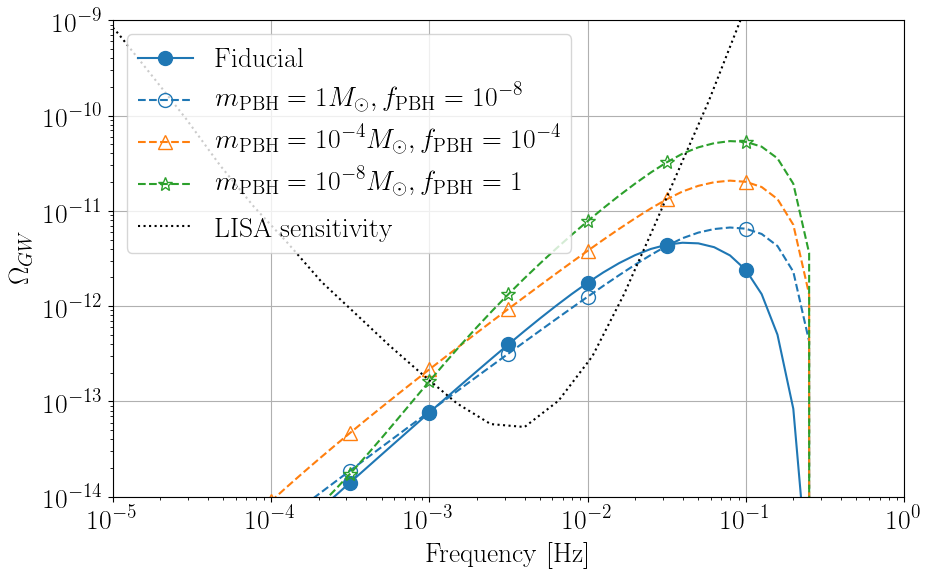
\includegraphics[width=\columnwidth]{GW-enhancement.png}
\caption{ A comparison between the \ac{SGWB} spectra with and without primordial \ac{BH} density enhancement effect due to \ac{GW} dissipation.
The fiducial model is calculated from the $\gamma=2$ dark-matter spike distribution for $m_\mathrm{PBH} = 1 M_\odot, f_\mathrm{PBH} = 10^{-8}$.
The three dashed lines are from the $\gamma=2$ enhanced dark-matter spike distribution due to \ac{GW} dissipation.
The mass and abundance parameters are so chosen to keep $m_\mathrm{PBH}f_\mathrm{PBH} = 10^{-8}$
}\label{fig:GWenhance}
\end{figure*}



\subsection{Modeling Systematics of the Massive Black Hole Population}\label{sec:robust}

To investigate the systematics on modeling the extragalactic massive \ac{BH} population, we vary the redshift integral limits, the lower mass of massive \acp{BH} and the massive \ac{BH} population model, respectively, and plot the corresponding \ac{SGWB} spectra.
The results are shown in \cref{fig:sgwbspace-robustness}. 
All \ac{SGWB} spectra are calculated from $\gamma=2$ dark-matter spike distribution and $f_\text{PBH} = 10^{-8}$, $m_\text{PBH} = 1 M_\odot$.

\subsubsection{The Redshift Limits of the Integral}

The left column of \cref{fig:sgwbspace-robustness} shows the \ac{SGWB} component contributions from different redshift ranges, $[0,1], [1,3]$ and $[3,5]$, respectively.
The fiducial result is the sum, i.e., obtained from the redshift range $[0,5]$.
We can see that the contribution from $z\in [3,5]$ is sub-dominant and accounts for at most $~10\%$ of the fiducial result.
We thus conclude that the choice of $5$ for the redshift upper limit is sufficient to capture the dominant contribution.

\subsubsection{The Lower Mass Cutoff of the Massive Black Holes}

As mentioned, we choose $10^4 ~h^{-1} M_\odot$ to be the minimum mass of massive \acp{BH} to account for the existence of such massive \acp{BH} from astronomical observations.
Nevertheless we change this value to $10^5 ~h^{-1} M_\odot$ to investigate the contribution from different mass ranges.
The result is shown in the middle column of \cref{fig:sgwbspace-robustness}.
Compared with the fiducial result whose lower mass cutoff is $10^4~h^{-1} M_\odot$, the result shows that the \ac{SGWB} contributed by $[10^4,10^5]~h^{-1} M_\odot$ massive \acp{BH} is mainly in the relative high frequency range $[\sim10^{-2}, \sim10^{-1}]$ Hz.
Therefore the shape of the \ac{SGWB} spectrum, especially the frequency of the peak, can provide information of the underlying massive \ac{BH} population. 

\subsubsection{The Population Model of Massive Black Holes}

A third investigation is to substitute the massive \ac{BH} population model derived from the \texttt{Reed07} dark-matter halo mass function to that proposed by Refs~.\cite{Barausse:2012fy,Sesana:2014bea,Antonini:2015cqa,Antonini:2015sza} accounting for the massive \acp{BH} formed from population III star seeds.
The number density of massive \acp{BH} of this model is
\be\label{eq:mbhpopiii}
\frac{dn}{d\log M_\mathrm{MBH}} = 0.005\( \frac{M_\mathrm{MBH}}{3\times 10^6 M_\odot}\)^{-0.3} \mathrm{Mpc^{-3}}
\ee 
The right column of \cref{fig:sgwbspace-robustness} presents the results.
It shows that the amplitude of the peak is one order of magnitude smaller than the fiducial model.
This is because the number density of massive \acp{BH} with mass $[10^4,10^6]~h^{-1} M_\odot$ from \cref{eq:mbhpopiii} is less than that from the \texttt{Reed07} derived population.

\begin{figure*}[htbp]
 %  figure placement: here, top, bottom, or page
   \centering
   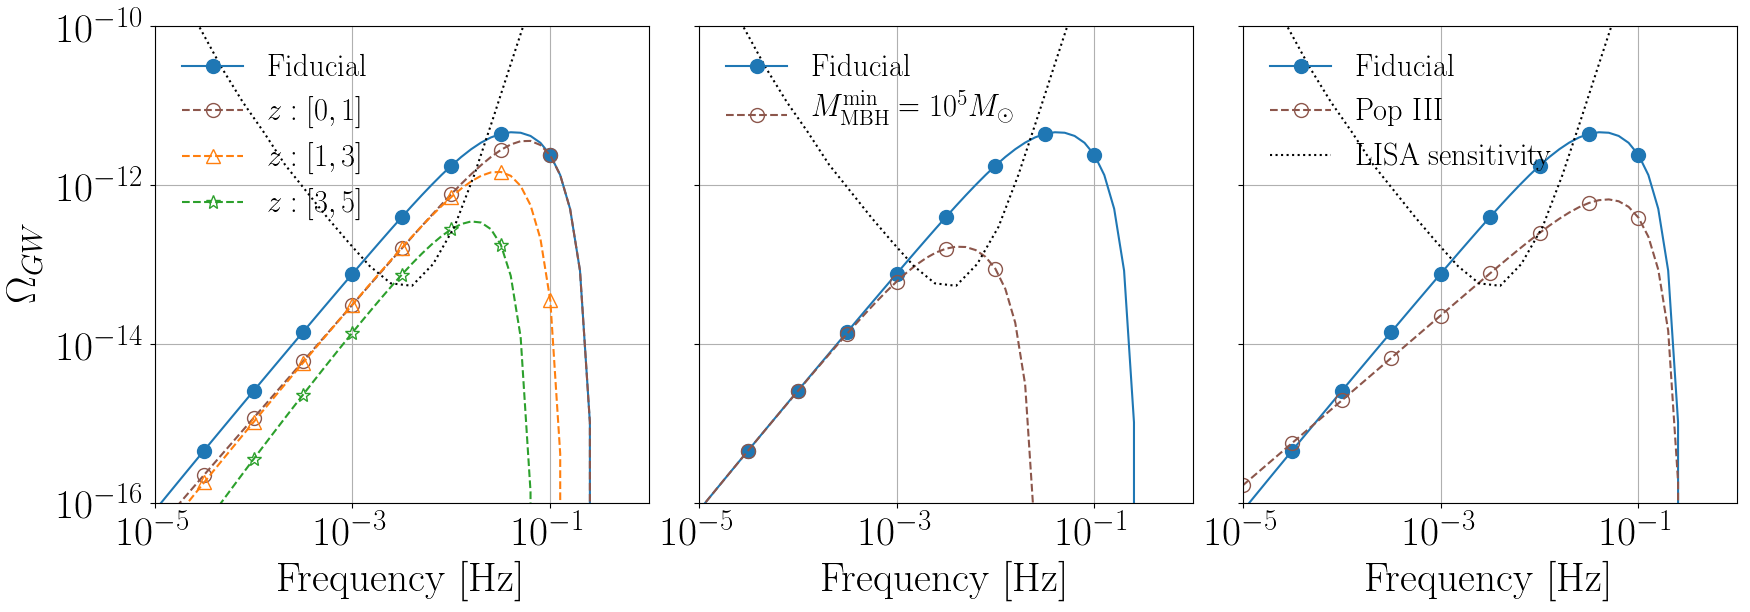
\includegraphics[width=\columnwidth]{0923-robust.png}
\caption{The effect on \ac{SGWB} spectra from the modeling systematics of massive \ac{BH}. 
The three figures present the \ac{SGWB} by varying the redshift integral limits, the lower mass of massive \acp{BH} and the massive \ac{BH} population model, respectively.
All \ac{SGWB} spectra are calculated from $\gamma=2$ dark-matter spike distribution and $f_\text{PBH} = 10^{-8}$, $m_\text{PBH} = 1 M_\odot$.}
\label{fig:sgwbspace-robustness}
\end{figure*}

The above investigations give a  quantitative measurement about the effect on \ac{SGWB} spectra from different modeling systematics of extragalactic massive \ac{BH}, which can be improved in the future once a better understanding of the population of massive \acp{BH} is obtained.
In addition, the future \ac{SGWB} search with space-based detectors can serve as a tool to probe the population information of massive \acp{BH}.

%%%%%%%%%%%%%%%%%%%%%%%%%%%%%%%%%%%%%%%%%%%%%%%%%%
\section{Constraints on Primordial Black Hole Abundance}\label{sec:PBH-EMRI-constraint}

By comparing the \ac{SGWB} spectrum with the LISA sensitivity and applying the condition
\be
\Omega_\text{GW}(\nu; m_\text{PBH}, f_\text{PBH} ) \leq \Omega_\text{GW}^\text{LISA sensitivity},
\ee
the upper limit on primordial \ac{BH} abundance $f^\text{max}_\text{PBH}$ can be obtained for a null searching result.
In \cref{Fig:constraints}, we plot the results for different primordial \ac{BH} masses from the models of $\gamma=1$, $\gamma=2$, with and without the enhancement due to \ac{GW} dissipation, respectively.
As a comparison, we also plot the current constraint from the microlensing search collaboration OGLE \cite{OGLE2019} and EROS \cite{EROS2006}.

It shows that LISA can probe the primordial \ac{BH} abundance in a large range of masses, $[10^{-9}, 1] M_\odot$ for  $\gamma=2$ and $[10^{-6}, 1] M_\odot$ for  $\gamma=1$, respectively. 
We do not consider more massive primordial \acp{BH} because it may break the condition of extreme mass ratio.
For primordial \acp{BH} with $1 M_\odot$, LISA can constrain the abundance to be $\sim10^{-6}$ ($\gamma=1$) or $\sim10^{-9}$ ($\gamma=2$). 
The enhancement effect due to \ac{GW} dissipation can further improve the constraint at the lower end of the mass range.
This would be the most sensitive method proposed and quantified by now for detecting or constraining sub-solar mass primordial \acp{BH}.

\begin{figure}[htbp]
 %  figure placement: here, top, bottom, or page
   \centering
   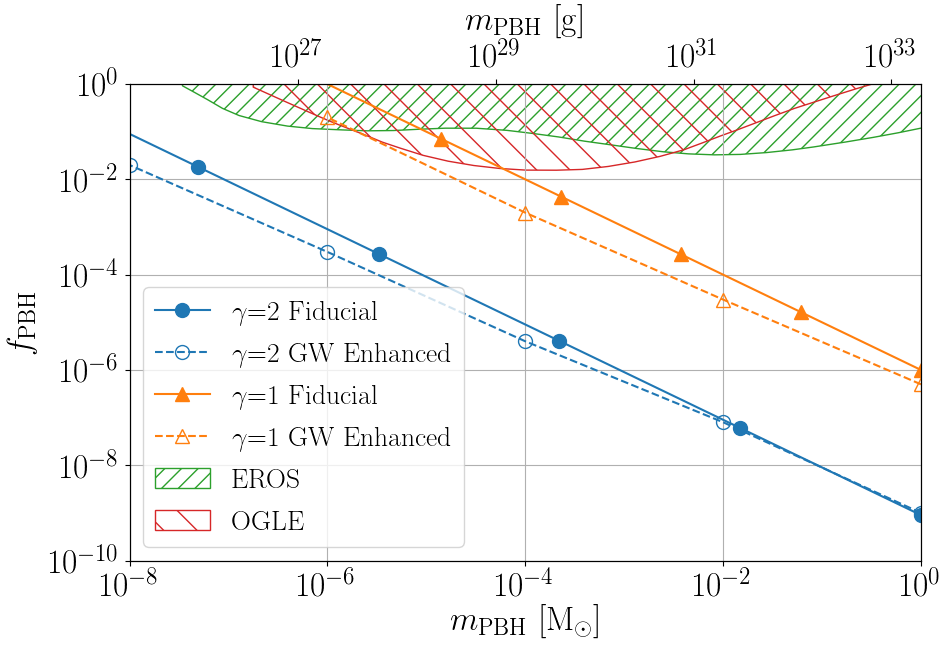
\includegraphics[width=\columnwidth]{0907constraint.png}
   \caption{The projected constraints on primordial \ac{BH} abundance in dark matter with \ac{LISA} for $\gamma=1$ and $\gamma=2$, with and without the enhancement due to \ac{GW} dissipation, respectively.
   As a comparison, we also plot the current constraint from the microlensing search collaboration OGLE \cite{OGLE2019} and EROS \cite{EROS2006}.
   }\label{Fig:constraints}
\end{figure}


\section{Conclusions and Discussions}\label{sec:PBH-EMRI-conclusion}

In this work we have investigated the \ac{SGWB} from primordial \ac{BH} \acp{EMRI} surrounding Sagittarius A$^\ast$ and the extragalactic massive \acp{BH}, respectively, expanding the previous work of Ref.~\cite{Kuhnel:2017bvu, SgrA} by including the complete extragalactic contribution.
After modeling the event rate, the \ac{SGWB} energy density spectra are calculated.
The contributions from Sagittarius A$^\ast$ peaks at $\sim 3\times 10^{-4}$ Hz and extragalactic massive \acp{BH} peak at $\sim 4\times 10^{-2}$ Hz.
%different characteristic frequencies.
Future space-based \ac{GW} detectors such as LISA may utilize this spectrum feature to distinguish different sources of \ac{SGWB} and give decisive evidence about the existence of primordial \ac{BH} dark matter at the galactic center.
Also note that the primordial \ac{BH} \ac{EMRI} around Sagittarius A$^\ast$ is a point source and the contribution from extragalactic is isotropic, therefore the directional and isotropic search for \ac{SGWB} \cite{SGWBlivingreview} should be employed for the above two kinds of signals, respectively.
However, the detailed data analysis formalism is beyond the scope of this work and left for a future work.

Finally, LISA can also constrain the abundance of primordial \ac{BH} in dark matter if there will be a null \ac{SGWB} searching result.
For a NFW induced dark-matter spike profile ($\gamma=1$), LISA can exclude the existence of $1 M_\odot$ primordial \ac{BH} with any abundance greater than $10^{-6}$ of dark matter.
A steeper dark-matter profile power index $\gamma=2$ can make the constraint even tighter by three order of magnitude.
This renders \acp{GW} in the space-based frequency band  a powerful tool to hunting for sub-solar mass primordial \acp{BH}.
However, modeling uncertainties exist from the dark-matter spike profile power index and the extragalactic massive \acp{BH} population as quantified in \cref{sec:extragalactic}.
Future astrophysical progress on understanding these modeling systematics can help further improve the ability of \ac{GW} window to search for primordial \acp{BH}.

\chapterend

\chapter{Outlook}\label{ch:outlook}

The field of \ac{GW} astronomy is moving forward very fast.
When writing this thesis, the third observation run of Advanced LIGO and Virgo is undergoing.
\ac{BBH} signals are detected weekly, \ac{BNS} and, especially,  \acl{NSBH} coalescence, for the first time, have possibly been identified.
Advanced LIGO and Virgo will further undergo upgrading towards the final design sensitivity.
The Japanese \ac{GW} detector KAGRA is expected to join the network soon before the end of the third observation run \cite{livingreviewligo}.
The India \ac{GW} detector is under construction.

More detectors, higher sensitivity, a greater number of data, all of them will allow to probe astrophysics with \ac{GW} to a new level.
The detection of \ac{SGWB} may also well happen in the near future.
Here we enumerate a few future directions related to the investigation of \ac{SGWB} and primordial \acp{BH} based on the work in this thesis.

\subsubsection{Anisotropic Stochastic Gravitational-Wave Background}

Recently, there is progress regarding the anisotropy of \ac{SGWB} of astrophysical origin.
Refs.~\cite{SGWBaniso1,SGWBaniso2,SGWBaniso3} derive the angular power spectrum for the \ac{SGWB} due to astrophysical \ac{BBH} coalescence. 

It has been shown by Ref~.\cite{Raccanelli:2016cud} that the correlation of \ac{GW} events with galaxy catalogs may distinguish the origin of \acp{BBH}, because the location of primordial \acp{BH} is not necessarily inside a galaxy.
Therefore, it could be interesting to investigate to what extent the binary primordial \acp{BH} coalescence can affect the anisotropy of \ac{SGWB}.
In other words, we can follow the work of \cref{chapter:sgwb-pbh} to probe the next-to-leading order, anisotropic \ac{SGWB} angular power spectrum.

\subsubsection {Waveforms for Binary Black-Hole Coalescence with Eccentricity}

The waveforms of \ac{GW} from eccentric \ac{BBH} merger have been developed recently by, e.g., Refs.~\cite{eccentric1,eccentric2,eccentric3,eccentric4,eccentric5,eccentric6,eccentric7}.

Since the binary primordial \acp{BH} form from dynamical interaction under the effect of tidal force exerted by a third body, the eccentricity can be non-zero.
Using the waveforms mentioned above, we can estimate the eccentricity with the existing \ac{GW} events and investigate the possible relationship between a non-zero value of eccentricity and the primordial \ac{BH} formation channel. 

\subsubsection{Directional Search for Stochastic Gravitational-Wave Background with Space-Based Detectors}

The directional search for \ac{SGWB} has been performed by Advanced LIGO and Virgo towards three directions, Scorpius X-1, Supernova 1987 A and the Galactic Center, respectively.
Corresponding upper limits have been given by Refs.~\cite{directional1,directional2,directional3}. 
As mentioned in \cref{chap:SGWBspace}, the data analysis framework for directional \ac{SGWB} search with space-based detectors is yet to be developed and quantified, from which the \ac{SGWB} constraints on primordial \ac{BH} \acp{EMRI} at the galactic center may be improved.

\appendix
%\input{a_inst}


%=======================================================

%bibliography
\bibliographystyle{ieee}
\bibliography{reference}



\end{document}
